\documentclass[12pt]{article}

% Packages
\usepackage[utf8]{inputenc}
\usepackage[english]{babel}
\usepackage[top=3cm,bottom=3cm,left=3cm,right=3cm,bindingoffset=0mm]{geometry}
\usepackage{amssymb}
\usepackage{amsmath}
\usepackage{subcaption}
\usepackage{tikz}
\usepackage{graphicx}
\usepackage{comment}
\usepackage{rotating}
\usepackage{float}
\usepackage{natbib}
\usepackage{amsthm}
\usepackage{bbm}
\usepackage{thmtools,thm-restate}
\usepackage{hyperref}
%\usepackage{extsizes}
\usepackage[font=footnotesize,labelfont=bf]{caption}

% New Options
\newtheorem{prop}{Proposition}
\newtheorem{definition}{Definition}[section]
\newtheorem*{remark}{Remark}
\newtheorem{lemma}{Lemma}
\declaretheorem{proposition}
\linespread{1.3}
\raggedbottom
\font\reali=msbm10 at 12pt

% New Commands
\newcommand{\real}{\hbox{\reali R}}
\newcommand{\realp}{\hbox{\reali R}_{\scriptscriptstyle +}}
\newcommand{\realpp}{\hbox{\reali R}_{\scriptscriptstyle ++}}
\newcommand{\R}{\mathbb{R}}
\DeclareMathOperator{\E}{\mathbb{E}}

\title{ICT and Future Productivity:\\Evidence and Theory of a GPT\thanks{Correspondence: Department of Economics, Boston College, 140 Commonwealth Avenue, Chestnut Hill, MA 02467. Email: brianti@bc.edu (Marco Brianti) and gati@bc.edu (Laura G\'ati).}}
\author{Marco Brianti \\ {\small Boston College} \and Laura G\'ati \\ {\small Boston College}}
\date{\today}


\begin{document}



\maketitle

\

\

\
%%%%%%%%%%%%%%%%%%%%             ABSTRACT           %%%%%%%%%%%%%%%%%% 
\small{
\abstract{We employ Structural VARs to investigate the effects of ICT supply shocks on Total Factor Productivity (TFP) and other macroeconomic variables. In response to this sector-specific supply shock, relative prices of ICT goods and services immediately fall, ICT investment rises on impact, and TFP displays a significant delayed and persistent increase. Taking up the view of theories of ICT as a general-purpose technology, we analyze a two-sector general equilibrium model in order to rationalize previous results and estimate spillovers from the stock of ICT via impulse-response matching. We conclude that ICT accumulation is able to enhance productivity through a positive spillover effect which takes into account the overall level of diffusion of ICT capital in the economy.}
}
\newpage



\newpage
%%%%%%%%%%%%%%%%%%%%               INTRODUCTION                 %%%%%%%%%%%%%%%%%% 
\section{Introduction}

Although there is large consensus on the importance of productivity as a driver of economic performance, there is less agreement on the underlying sources of productivity growth. For several years, much of the business-cycle literature decided to avoid such questions by proxying movements in productivity by exogenous shocks.\footnote{\cite{kydland1982time} and \cite{long1983real} are among the first papers which consider productivity shocks in general equilibrium models.} However, the robust empirical evidence of the slowdown in productivity right before the Great Recession has led recent literature to take a step back and devote more attention to the drivers of medium-term productivity growth.\footnote{See \cite{cette2016pre} and \cite{byrne2016does} among others.}

Along with \cite{comin2006medium}, theoretical contributions rationalize endogenous productivity dynamics by incorporating features of endogenous growth models in standard models of business cycles. Following \cite{romer1990endogenous}, most of these papers augment final-good production functions with an expanding composite of intermediate goods invented by the Research \& Development (R\&D) sector in order to allow for an endogenous rate of adoption of new technologies.\footnote{\cite{bianchi2014growth}, \cite{anzoategui2016endogenous}, and \cite{moran2017innovation} use similar techniques to endogenize growth. \cite{bianchi2014growth} augment a DSGE  model using a quality ladders model in the vein of \cite{grossman1991quality}. \cite{anzoategui2016endogenous} and \cite{moran2017innovation}, similarly to \cite{comin2006medium}, use a model of expanding variety \`a la \cite{romer1990endogenous}.} Guided by the prediction of such theoretical work that R\&D developments matter for growth, other papers attempt to provide empirical evidence of a slowdown in the productivity of the R\&D sector. Specifically, they show that although research effort keeps rising, the rate of new ideas and discoveries is slowing down.\footnote{\cite{jones2009burden} and \cite{bloom2017ideas} are two contributions that highlight these facts.}

Motivated by this wave of research, this paper follows a different path and argues that Information and Communication Technology (hereafter ICT) plays an important role in driving medium-term productivity in sectors that are ICT users. Our contribution is twofold. First, we provide robust empirical evidence to show that current rises in ICT investment explain significant and persistent increases in future Total Factor Productivity (hereafter TFP). Second, we analyze a standard theoretical framework in order to both rationalize our empirical results and to draw conclusions concerning the nature of the ICT contribution to future productivity. 

In the empirical section, we identify technological shocks specific to the ICT sector in a Structural VAR context.\footnote{An interesting paper related to our empirical work is \cite{jafari2012impact}. The authors identify ICT shocks as a potential driver of the Iranian business cycle using a completely different identification strategy and obtaining qualitatively different results.} Our multivariate system includes three key variables: TFP, ICT investment (hereafter ICTI), and relative prices (hereafter RP). ICTI is defined as the total expenditure in equipment and computer software meant to be used in production for more than a year. Thus, an increase in ICTI is ICT capital deepening. RP is the ratio between the price level of ICT durable goods and the price level in the overall economy. 

We use two identifying restrictions in order to back out an ICT technology shock. First, we expect it to be orthogonal to the current productivity of all the other sectors. Since the share of the ICT sector accounts for a negligible part of the whole economy, ICT shocks should have an approximately zero effect on TFP on impact. Thus, our first restriction will be a zero-impact restriction on TFP after an ICT shock. Moreover, following \cite{greenwood1997long} and \cite{fisher2006dynamic}, we rely on RP and ICTI because we expect that a sectoral technology shock should decrease the relative prices of the sector while enhancing expenditure in the underlying sector. For theoretical reasons discussed in more detail below, we do not impose any restriction on RP; instead, we let the ICT shock maximize the impact response of ICTI.\footnote{As pointed out by both \cite{greenwood2000role} and \cite{basu2010sector}, letting the the direction of RP be the sole identifying restriction does not properly capture technological changes between sectors. This is the main reason why we do not impose the direction of RP as a direct identifying condition. While our main robustness check uses RP, also there we refrain from considering the direction of the RP response. See Section \ref{section:twosteps}.} In response to this shock, ICTI rises on impact and remains significant for several quarters. RP persistently and significantly declines for more than two years, suggesting that we are indeed identifying the correct sectoral shock. Our main result is that TFP, restricted not to respond on impact, rises after few quarters and remains significant and stable for at least 5 years, despite the tiny size of the ICT sector relative to the economy. Finally, variance decomposition analysis suggests that ICT shocks explain a remarkable size of economic fluctuations over the medium and long run. These shocks drive about $40$\% and $33$\% of the overall GDP and TFP fluctuations over a 10-year horizon, respectively.

Although our results are robust over different specifications, a critique to our empirical strategy is reverse causality coming from news on future TFP. As suggested by the news-shock literature, the positive reaction of ICTI on impact may be triggered by signals related to future increases in TFP and not to contemporaneous ICT technological improvements. In other words, our identification strategy may confound our shock of interest with a news shock which contemporaneously enhances investment in ICT capital goods. We address this issue by providing a series of alternative identification strategies which we show deliver the same time series of ICT innovations as our initial specification. The heart of these robustness checks is sequential identification of news and ICT shocks: we first identify a news shock in the spirit of \cite{barsky2011news}, and subsequently we identify our sectoral ICT shock using the previous identification strategy. Encouragingly, controlling for signals regarding future movements in TFP does not affect our results. We view this as strengthening the causality relation from current ICT investment to future TFP. 

In order to understand the economics behind our empirical results, we then analyze a two-sector DSGE model which allows ICT to be the general-purpose technology (hereafter GPT) of the whole economy. There are two main justifications for interpreting ICT as a GPT. On the one hand, there is a vast literature that makes a case for the general-purpose nature of ICT capital.\footnote{See for example \cite{oliner2000resurgence} and \cite{stiroh2002information} amongst others.} On the other hand, the tiny share of the ICT sector both in overall investment and overall output makes our results of a strong and persistent TFP increase after an ICT shock hard to interpret in absence of an additional force such as an externality coming from the general-purpose property of ICT capital.

In our model, both sectoral production functions are fed with three inputs: (i) labor, supplied by households, (ii) hard capital, produced by the final sector, and (iii) ICT capital, produced by the ICT sector. As explained by both \cite{basu2003case} and \cite{basu2007information}, a GPT should be able to enhance accelerations in productivity in sectors that are users of the underlying technology. We then interpret ICT as the GPT of the last 30 years of the U.S. economy assuming that exogenous technological changes in the ICT sector are able to affect economy-wide productivity above the direct effect coming from the technology increase itself.\footnote{A clarification is in place here. In a two-sector model, total factor productivity is a convolution of the two exogenous productivities. Thus sectoral productivity changes trivially show up in TFP as a direct effect. Our assumption of ICT capital being a GPT means that overall productivity responds much more to an ICT-sector-specific technology shock than warranted by this shock directly. We address this question in detail in the main text in Section \ref{section:empirics}.} In particular, when an ICT technology shock arrives, both sectors accumulate ICT capital since it is easier to produce and cheaper to buy. This ICT capital deepening consequently enhances the productivity of both sectors by means of a spillover coming from the accumulated ICT capital stock. 

What is the intuition behind our assumption of ICT as a GPT showing up in the economy as a spillover? To better understand this externality assumption, consider the special nature of ICT capital. Since the purpose of ICT capital is to improve information acquisition and sharing, the quality and speed of communication fundamentally depends on the diffusion of these technologies among agents. As a simple example, owning a mobile phone enables one to contact another person instantaneously only if the other person is also endowed with the same technology. As a result, the effectiveness of ICT capital is intrinsically related to its own diffusion. This line of thought is what leads us to augment the production function of each sector with a spillover effect capturing the diffusion of ICT capital.  Having a spillover arise from a state variable is also consistent with both the GPT literature above and with our empirical results, since it also leads to model dynamics in which the accumulation of ICT capital is a slow process and the benefits of an ICT technology shock show up in the production functions of ICT-users with lags.\footnote{Notice that differently to \cite{basu2003case} and \cite{basu2007information}, we interpret the general-purpose nature of ICT in the spirit of an endogenous growth model.}

As a last step, we use both our empirical and theoretical results to estimate the key parameters of the model via impulse-response matching to an ICT technology shock. The key parameters are (i) the elasticity of productivity to ICT capital diffusion, namely the parameter which governs the spillover effect, and (ii) the standard deviation and (iii) persistence of ICT technology shocks. Results consistently obtain a positive spillover effect of ICT capital deepening on TFP, confirming that within this class of theoretical models, data supports the existence of spillovers from ICT capital. Thus, our theoretical model suggests to interpret the responses obtained in the empirical section in light of ICT as a general-purpose technology which enhances productivity of ICT capital users through a spillover effect related to its own diffusion.

\begin{comment}
Our paper is mainly related to three strands of literature. First of all, we link to the literature that investigates the recent slowdown in TFP growth. Our project is motivated by papers such as \cite{oliner2007explaining}, \cite{jorgenson2008retrospective}, \cite{byrne2016does}, \cite{cette2016pre}, and \cite{fernald2017disappointing} who document that the slowdown in TFP growth occurred before the recession implying that the financial crisis per se cannot be its cause.\footnote{In particular, in line with our results, also \cite{fernald2017disappointing} conclude that the pause in the information technology revolution is the main candidate explanation.} Secondly, our project is related to the literature that investigate the effects of investment-specific technology shocks in a multi-sector economy. In particular, throughout the paper our main references will be \cite{greenwood1997long}, \cite{oulton2007investment}, and \cite{fisher2006dynamic}. However, both the empirical exercise and the theoretical model are strictly related to \cite{greenwood2000role}, \cite{basu2010sector}, and \cite{justiniano2011investment}. Finally, this paper is also related to papers that argue that information and communication technology is the current general-purpose technology. Main references will be bresnan, and \cite{basu2007information}.
\end{comment}

The paper is structured as follows. We present empirical results and main robustness checks in Section \ref{section:empirics}. We then present and analyze the two-sector DSGE model in Section \ref{section:theory}. We estimate via impulse-response matching key parameters of the model and assess its empirical reliability in Section \ref{section:model_assessment}. Section \ref{section:conclusions} concludes.



%%%%%%%%%%%%%%%%%%%%%%            EMPIRICS                     %%%%%%%%%%%%%%%%%%%
\section{Empirics}\label{section:empirics}

In this section we present our main empirical results. Our attempt is to properly identify technological shocks which are specific to the ICT sector in a Structural VAR context and to analyze their impact on key macroeconomic variables.

\subsection{Main Specification}\label{section:mainSpec}

We start by illustrating our main specification where we impose minimal discipline on the model. In subsequent sections, we try vastly different empirical strategies. It turns out that the set of results presented here are consistent with the different robustness checks.

\subsubsection{Data}

Our first-step specification is the following five-variable VAR 
\begin{equation}\label{eq:mainSpecification}
\begin{pmatrix}
TFP_t \\ 
ICTI_t \\
GDP_t \\
C_t \\
RP_t \\
\end{pmatrix} = B(L) \begin{pmatrix}
TFP_{t-1} \\ 
ICTI_{t-1} \\
GDP_{t-1} \\
C_{t-1} \\
RP_{t-1} \\
\end{pmatrix} + i_t
\end{equation}
where $TFP_t$ is the log-level of Fernald total factor productivity at time $t$, $ICTI_{t}$ is the log-level of real information and communication technology investment at time $t$,\footnote{$ICTI_t$ is defined as the total expenditure at time $t$ in equipment and computer software meant to be used in production for more than a year.} $GDP_t$ is the log-level of real gross domestic product at time $t$, $C_t$ is the log-level of real consumption at time $t$, and $RP_t$ is the log-deviation of the ratio between prices of ICT goods and services and the consumer price index (CPI).\footnote{Except for $RP_t$, which is not cointegrated with the remaining variables, we opt for estimating the VAR in levels since this produces consistent estimates of the impulse responses and is robust to cointegration of unknown forms. In particular, as suggested by \cite{hamilton1994time}, when there is uncertainty regarding the nature of common trends, estimating the system in levels is considered the conservative approach. The alternative approach is to estimate the system as a vector error correction model (VECM); our results remain very similar also in this case.} \footnote{Using the PCE deflator instead of the CPI yields similar results.} Our dataset is quarterly and covers the U.S. economy from 1989:Q1 to 2017:Q1.\footnote{All data are from the BEA except for TFP, which is the series constructed by John Fernald, available on his website.} $B(L)$ is a ($5\times 5$) matrix of lag-operator functions of the same order. Following the Bayesian Information Criterion (BIC), we choose one lag, which implies that we regress variables at time $t$ with their own lagged values at $t-1$.\footnote{The Hannan-Quinn Criterion (HQ) suggests to use two lags. Results remains consistent following this second criterion.} Finally, $i_t$ is a ($5 \times 1$) vector of correlated innovations where $\Sigma = i'_t i_t$.

\subsubsection{Empirical Strategy}\label{section:empiricalstrategy_simple}


Our simplest identification strategy assumes that an ICT technological shock (hereafter ICT shock) has (i) no impact effect on TFP and (ii) maximal impact effect on ICTI. We justify these two assumptions with both empirical and theoretical arguments. First of all, as data released in April, 2018 by the Bureau of Economic Analysis (BEA) shows, the real value added of the information sector on real GDP is slightly below $5$\% for the underlying quarter.\footnote{There are many ways to quantify the size of the ICT sector, both in terms of what share one considers and how one defines the ICT sector. The number in the text refers to the value added share of the ICT sector, defined as in Section \ref{eq:mainSpecification}. The statement that the ICT sector is tiny is however not sensitive to the definition of the sector or to the choice of share. Even with broader definitions, one obtains numbers in the range of 5\%.} Thus, since the ICT sector accounts for a negligible part of the whole economy, we think it is safe to assume that an ICT shock is orthogonal to current TFP. 

In addition, the theory of multi-sector models, as presented by \cite{greenwood1997long}, predicts that a productivity increase in one sector should lead to sectoral output becoming cheaper. Thus, we expect that an ICT shock should enhance sector-specific investment since ICT goods are less costly to produce and to buy. As a result, we expect an ICT shock to have a maximal impact effect on ICTI. 

Using a notation similar to \cite{barsky2011news}, we implement our identification strategy as follows. Let $y_t$ be the $(5 \times 1)$ vector of observables of length $T$ presented above. The reduced-form VAR takes the following form,
$$
y_t = B(L)y_{t-1} + i_t 
$$
Assume now that there exists a linear combination that maps innovations $i_t$ to structural shocks $s_t$,
$$
A_0 s_t = i_t
$$
which implies the structural-form VAR
$$
A_0^{-1}y_t = C(L) y_{t-1} + s_t
$$
where $C(L) = A_0^{-1} B(L)$ and $s_t = A_0^{-1} i_t$. The impact matrix $A_0$ must be such that $\Sigma = A_0 A_0'$. Notice that $A_0$ is not unique since for any $D$ such that $DD' = I$, $\tilde{A}_0 = A_0 D$ satisfies $\Sigma = \tilde{A}_0 \tilde{A}_0'$. 

The matrix of impact responses to all shocks is: % TYPO HERE? either Atilde or A0 D. Checked Barsky, this seems correct but I'm confused. 
$$
\Pi(0) = \tilde{A}_0 D
$$
and is specifically formed by the following elements, denoting the responses of variable $i$ to shock $j$, % same here
$$
\Pi_{i,j}(0) = e_i' \tilde{A}_0 D e_j
$$
where $e_k$ is a selector column vector of the same dimension as $\tilde{A}_0$ with $1$ in the $k$th element and zero elsewhere. In particular, notice that $e_j$ is selecting a specific column of $D$. Let this column be denoted by $\gamma_j$. Using this notation, $\tilde{A}_0\gamma_j$ is the vector of impact responses of all the variable to shock $j$.

Observe from System \ref{eq:mainSpecification} that $TFP_t$ is ordered first and $ICTI_t$ second. Our identification strategy is then the solution to the following problem:
\begin{equation}\label{eq:mainObjective}
\max_{\gamma_j} \Pi_{2,j}(0) = e_2' \tilde{A}_0 \gamma_j
\end{equation}
subject to
\begin{equation}\label{eq:mainZeroTFP}
\Pi_{1,j}(0) = e_1' \tilde{A}_0 \gamma_j = 0, \ \ \text{and}
\end{equation}
\begin{equation}\label{eq:mainOrtho}
\gamma_j' \gamma_j = 1
\end{equation}
where $j$ represents the arbitrary position of the ICT shock. Then, in order to ensure that this identification belongs to the space of possible orthogonalizations of $\Sigma$, the problem is formulated in terms of choosing $\gamma_j$ conditional on any orthogonalization, $\tilde{A}_0$. Objective function \ref{eq:mainObjective} imposes that an ICT shock has a maximal impact effect on ICT investment. Constraint \ref{eq:mainZeroTFP} orthogonalizes current TFP to ICT shocks and Constraint \ref{eq:mainOrtho} satisfies the condition that $\gamma_j$ is derived from an orthogonal matrix $D$.  

\subsubsection{Main Set of Results}

Appendix \ref{section:mainSetResults} shows the estimated impulse responses of System \ref{eq:mainSpecification} to the identified ICT shock. The shaded gray areas are the $90$\% and $95$\% confidence bands from the bias-corrected bootstrap procedure of \cite{kilian1998small} using 2000 simulations. Our main interest, Figure \ref{fig:TFP_main}, shows the impulse response of TFP to an ICT shock. TFP takes around $4$ quarters before displaying a positive and significant effect and reaches its peak of $1.2$\% after $24$ quarters. In Figure \ref{fig:ICT_main}, real ICT investment has a large and positive impact response of almost $2$\% that gets even larger after a quarter. Then, it slowly starts to decay, remaining significant for more than $40$ quarters. In Figures \ref{fig:GDP_main} and \ref{fig:C_main}, we present responses of real GDP and real consumption, respectively. Real GDP has a significant impact response of $0.3$\% and reaches its peak of almost $0.5$\% approximately at the same time as TFP. Similarly, real consumption has an impact effect of $0.2$\% with a delayed peak of $0.5$\%. Finally,  Figure \ref{fig:RP_main} depicts that response of relative prices. Despite imposing no restriction here, the response of RP is broadly in line with multi-sector theory. Relative prices drop significantly on impact by $0.4$\% and remain persistently below their own steady state value for almost $9$ years.

In addition, Table \ref{table:vardec} in Appendix \ref{section:vardec} presents forecast error variance decompositions for the ICT shock on each variable. The table shows decompositions on impact, and at a one-, two-, four-, six-, and ten-year horizon. These results are very interesting in their own right, as they hint that the ICT sector may have a particular role for the overall productivity of the economy. In line with the impulse responses, ICT shocks, which are orthogonal to current productivity, explain nothing of current TFP fluctuations. At a ten-year horizon, however, this fraction is over a third! This crucial result is a strong sign that the ICT sector matters for overall productivity over and beyond the direct contribution of its sectoral productivity (which, as we have seen, is marginal). At the same time, ICT shocks drive almost the whole variation in ICT investment on impact, with a slow decay over time to below $50$\% after 10 years. Interestingly, both output and consumption have a remarkable reaction on impact: $26$\% and $19$\%, respectively. Moreover, this effect tends to increase, reaching $40$\% in both cases at the maximal horizon. Finally, ICT shocks only account for a small fraction of movements in relative prices. The fraction of fluctuations explained on impact is only $6$\% with a peak of $14$\% between four and six years. Overall, these variance decompositions all seem to suggest that the ICT shock leads to complex forms of reallocation and accumulation that take place over the medium run in the economy and that seem to result in productivity growth. Our structural model of Section \ref{section:theory} provides a theoretical framework to think about these dynamics and to give them an economic interpretation. 

\subsection{Controlling for News Shocks}

In this section, we present a set of robustness checks aimed to show that our previous results are not driven by future signals regarding exogenous productivity. The main concern against the specification of \ref{section:mainSpec} is reverse causality coming from the presence of news about future TFP that is not accounted for. Indeed, the news-shock literature warns that the positive reaction of ICTI on impact may be triggered by signals related to future increases in productivity and not to a contemporaneous ICT shock. In other words, our identification strategy may confound our shock of interest with a news shock which contemporaneously enhances investment in ICT capital goods. We address this issue by providing two main alternative identification strategies which we show deliver the same time series of ICT shocks as our initial specification. 

As a first-pass test, % cite Barsky Basu Lee and Forni or whatevs
we check if our results are robust once we remove all the forward-looking variables whose fluctuations may be unrelated to sector-specific technological changes: consumption and output. Technically speaking, consumption and output may Granger-cause movements in future TFP for reasons which are orthogonal to ICT shocks. For example, the forward-looking nature of consumption may provide the VAR with information regarding future changes in TFP not related to an ICT shock, which our identification strategy is not able to filter out. 

Our second and main robustness test is running a VAR in which we identify both ICT shocks and news shocks. In particular, we apply a sequential identification where we first identify a news shock in the spirit of \cite{barsky2011news}, and subsequently we identify our sectoral ICT shock using our original identification strategy. This second strategy has the specific purpose of directly filtering out all the current movements in forward-looking variables related to future fluctuations of TFP which are not related to current ICT shocks, as such fluctuations are all captured by the identified news shock.

As is illustrated in the rest of this section, both our robustness checks recover the same series for structural ICT shocks as our initial specification, and thus leave our results unaffected. We therefore conclude that controlling for signals regarding future movements in productivity does not affect our identified ICT shocks, and thus confirm the causal relation between current ICT investment and future TFP.

\subsubsection{Removing Forward-Looking Variables}\label{sec:removing}

We now show our first-pass test in detail. As discussed by \cite{sims2012news}, \cite{forni2014sufficient} and \cite{barsky2015whither}, the presence of forward-looking variables in the VAR is a necessary condition to correctly identify a news shock. In particular, since the univariate TFP process cannot predict its own future values,\footnote{It is well-accepted that TFP growth can be approximated as a white noise process.} a news shock can only be identified if there are variables that Granger-cause TFP inside the VAR. For example, \cite{beaudry2006stock} use current movements in stock prices to predict future productivity, but also contemporary fluctuations in consumption, hours, investment, may implicitly reflect information regarding future technical change.

Thus, as a simple test, we redo the exercise described in Section \ref{section:mainSpec}, omitting the two forward-looking macroeconomic variables not directly related with the ICT sector: consumption and output.\footnote{Note that output implicitly reflects the behavior of hours and investment once we control for consumption.} If we are actually confounding news shocks with our ICT shock series then we would expect to see some differences in this second estimate, because absent the two forward-looking variables, our VAR is deprived of a source of information useful to recover a news shock and should thus no longer be able to capture it appropriately.

Without consumption and output, we thus estimate the following three-dimensional system
\begin{equation}\label{eq:noForVariables}
\begin{pmatrix}
TFP_t \\ 
ICTI_t \\
RP_t \\
\end{pmatrix} = B(L) \begin{pmatrix}
TFP_{t-1} \\ 
ICTI_{t-1} \\
RP_{t-1} \\
\end{pmatrix} + i_t
\end{equation}
where  $TFP_t$, $ICTI_{t}$, and $RP_t$ are defined and treated as in System \ref{eq:mainSpecification}. As before, the dataset is quarterly and covers the U.S. economy from 1989:Q1 to 2017:Q1. Finally, analogously to before, we follow the Bayesian Information Criterion (BIC) to choose one lag. Using the same identification strategy presented in \ref{section:empiricalstrategy_simple}, we recover a series of ICT shocks. The newly recovered series is correlated at $95$\% with the one estimated in the five-dimensional system, indicating that our main specification is not contaminated by news. Figure \ref{fig:shockSeries_removing} in Appendix \ref{section:removing_FL_Var} shows the ICT shock series for both the three-dimensional system and the five-dimensional one. In line with the very high correlation coefficient, the two series overlap perfectly, suggesting that both procedures recover the same structural shock series. Thus, our first-pass test indicates that our initial result is not driven by the forward-looking power of consumption and output on TFP. 

However, although this result is encouraging, the first-pass test has weak power because the jump of ICTI on impact may itself be triggered by exogenous signals on future TFP. In this case, ICTI would be itself the source to Granger-cause TFP and our ICT shock would be upward biased by news. To address this deeper concern, we proceed to employ a more complicated strategy aimed at directly capturing and filtering out news. 


\subsubsection{Sequential Identification Strategy}\label{section:twosteps}

We now turn to an alternative procedure to rule out the presence of news from our recovered ICT shock. In this second test we run a VAR where we identify both ICT shocks and news shocks. In contrast to our first-pass test, this approach aims to directly identify and filter out future signals unrelated to current ICT shocks.

We apply a sequential identification which involves first identifying a news shock in the spirit of \cite{barsky2011news}, and subsequently identifying the ICT shock using our original strategy. Specifically, in the first step the news shock is identified as the shock orthogonal to current TFP that best explains its future movements. Then, as a second step, the ICT shock is identified as the shock orthogonal to current TFP that maximizes the impact effect on ICT investment. 

However, in order to correctly employ this procedure, we need to take care of a second issue. As \cite{barsky2011news} warns, 

\begin{quote} A general objection to our emprical approach would be that a number of structural shocks, which are not really news in the sense defined in the literature, might affect a measure of TFP in the future without impacting it immediately. Among these shocks might be research and development shocks, investment specific shocks, and reallocative shocks. Our identification (and any other existing VAR identifications) would obviously confound any true news shock with these shocks. %add p. number
\end{quote}

\hspace{9cm} \cite{barsky2011news}, p. 278.

\vspace{0.5cm}

In other words, by naively employing the procedure presented above, any ICT shock would be interpreted as a news shock since it is orthogonal to current TFP and explains its future movements. Put plainly, to get the identification of the two shocks right, we need to add a restriction that is able to distinguish between them.

Thus, to avoid confounding ICT shocks with news shocks, we need to augment the first step with an extra restriction. The restriction we will use here is derived from a two-sector structural model in the tradition of \cite{greenwood1997long}.\footnote{While our model belongs to the class of models along the lines of \cite{greenwood1997long}, our exposition is closer to that of \cite{oulton2007investment}. We discuss this choice in detail in Section \ref{section:theory}.} Here, we refrain from presenting the model in its entirety; the reader is referred to Section \ref{section:theory}. Instead, Proposition \ref{prop:priceRestriction} presents the key property of the model that gives rise to our identification assumption. 

\begin{prop}\label{prop:priceRestriction}
In a two-sector economy, if both production functions display identical input shares, then any economy-wide productivity shocks do not affect relative prices between the two sectors.
\end{prop}
\begin{proof}
	See Appendix \ref{section:proofpriceRestriction}.
\end{proof}

Proposition \ref{prop:priceRestriction} implies that an anticipated future sector-neutral technological change (the so-called news shock) never affects relative prices between sectors. Obviously, this statement is correct under the extreme assumptions that (i) the shock is expected to have the same impact on the two sectors and (ii) production functions have identical input shares. If those assumptions hold in the data, then the correct additional restriction would be to  restrict the impulse response of relative prices to a news shock to hard zero at all horizons. However, this restriction would obviously penalize the identification of news shocks since it is unlikely that assumptions (i) and (ii) perfectly hold in the data. We therefore opt for a more moderate strategy where we impose that the impulse response of relative prices to news should be zero on some specific horizons rather than at all horizons. While results are robust to different horizon restrictions, our favorite specification is the one which sets relative prices to have zero response in the first three periods. 

\subsubsection*{Data}

Motivated by Section \ref{sec:removing}, we augment our initial VAR system with stock prices in order to provide an additional forward-looking variable to the system. Thus, our current specification is the following six-variable VAR,
\begin{equation}\label{eq:newsSpecification}
\begin{pmatrix}
TFP_t \\ 
SP_t \\
ICTI_t \\
GDP_t \\
C_t \\
RP_t \\
\end{pmatrix} = B(L) \begin{pmatrix}
TFP_{t-1} \\ 
SP_{t-1} \\
ICTI_{t-1} \\
GDP_{t-1} \\
C_{t-1} \\
RP_{t-1} \\
\end{pmatrix} + i_t
\end{equation}
where $TFP_t$, $ICTI_t$, $GDP_t$, $C_t$, and $RP_t$ are defined and treated identically to System \ref{eq:mainSpecification}. $SP_t$ represents the log-transformation of Standard \& Poor's 500 stock price index.  As before, the dataset is quarterly and covers the U.S. economy from 1989:Q1 to 2017:Q1 and following the BIC and HQ criteria we choose one lag.

\subsubsection*{Empirical Strategy}

Using the notation of Section \ref{section:empiricalstrategy_simple}, assume for simplicity that $B(L) = B$ allows for only one lag. Define the impulse response of variable $i$ to the identified shock $j$ at time $t$ as,\footnote{We also suppress the constant to simplify the notation. Of course, our identification strategy can be applied for $B(L)$ allowing for more than one lag and with the constant.}
$$
\Pi_{i,j}(t) = e_i' B^t \tilde{A}_0 D e_j = e_i' B^t \tilde{A}_0 \gamma_j
$$
and its variance decomposition up to time $h$ as
$$
\Omega_{i,j}(h) = \frac{ \sum_{t=0}^h e_i' B^t \tilde{A}_0 D e_j e_j' D' \tilde{A}_0' B'^t e_i } {e_i'( \sum_{\tau = 0}^H B^t \Sigma B'^t )e_i} = \frac{ \sum_{t=0}^h e_i' B^t \tilde{A}_0 \gamma_j \gamma_j' \tilde{A}_0' B'^t e_i } {e_i'( \sum_{\tau = 0}^H B^t \Sigma B'^t )e_i}
$$
Given this and recalling that TFP is ordered first, ICTI second and RP sixth, the identification strategy can be summarized as follows,

\subsubsection*{Step 1 - Identification of $\gamma_{news}$}
$$
\max_{\gamma_{news}} \Omega_{1,news}(h) = \frac{ \sum_{t=0}^h e_1' B^t \tilde{A}_0 \gamma_{news} \gamma_{news}' \tilde{A}_0' B'^t e_1 } {e_1' ( \sum_{\tau = 0}^H B^t \Sigma B'^t )e_1}
$$
subject to
$$
\Pi_{1,news}(0) = 0,
$$
$$
\Pi_{6,news}(0) = \Pi_{6,news}(1) = \Pi_{6,news}(2) = 0, \ \ \text{and}
$$
$$
\gamma_{news} \gamma_{news}' = 1.
$$
where the first constraint represents the zero-impact restriction of news on TFP. The second constraint is the restriction derived from Proposition \ref{prop:priceRestriction} to have the response of relative prices to news relatively small.\footnote{Our identification strategy is robust to different restrictions to relative prices. Results hold if we set the zero restriction on other horizons.} Finally, the last constraint imposes that $\gamma_{news}$ should be a column derived from the orthogonal matrix $D$. 


\subsubsection*{Step 2 - Identification of $\gamma_{ICT}$}
$$
\max_{\gamma_{ICT}} \Pi_{2,ICT}(0) =  e_2' \tilde{A}_0 \gamma_{ICT} 
$$
subject to
$$
\Pi_{1,ICT}(0) = 0,
$$
$$
\gamma_{news} \gamma_{ICT}' = 0, \ \ \text{and} \ \ \gamma_{ICT} \gamma_{ICT}' = 1.
$$
where the first constraint represents the zero-impact restriction of ICT on TFP and the last constraint imposes that both $\gamma_{news}$ and $\gamma_{ICT}$ should be two different columns derived from the orthogonal matrix $D$.

\subsubsection*{Results}

Figures \ref{fig:2stepIRF_first} and \ref{fig:2stepIRF_second} in Appendix \ref{section:IRF_2step} show estimated impulse responses to both news and ICT shocks. Figure \ref{fig:2stepIRF_first} focuses on the responses of TFP, stock prices, and ICT investment, while Figure \ref{fig:2stepIRF_second} shows the responses of GDP, consumption and relative prices. The shaded gray areas are the $90$\% and $95$\% confidence bands from the bias-corrected bootstrap procedure of \cite{kilian1998small} using 2000 simulations. 

A first comforting indication is that the responses to an ICT shock are almost identical to the ones from our main identification of Section \ref{section:mainSpec}. After few lags, TFP displays a positive and significant response and reaches its peak of $1.2$\% after $6$ years. Interestingly, stock prices jump on impact and the effect remains significant over the medium run. Real ICT investment has a large and positive impact response and slowly starts to decay, remaining significant for a long period of time. Both real GDP and real consumption have a significant impact response and reach their peak approximately after $6$ years. The response of relative prices is negative and persistent as we have previously discussed. Finally, the ICT shocks explains $27$\% of TFP fluctuations over a $10$-year horizon. Also this result is completely in line with the previous results presented in Table \ref{table:vardec} in Appendix \ref{section:vardec}.

In addition, we show the impulse responses to a news shock to confirm that our identification strategy is picking up news shocks correctly (left panel of the same figures). As the figures depict, constraining the response of relative prices to news does not qualitatively affect the behavior of news shocks; our identified news shock generates responses broadly in line with those found by the news shock literature. In particular, in line with \cite{barsky2011news}, it takes more that 2 years after the news shock for TFP to display a positive, significant and strongly persistent effect. Stock prices have a strong forecasting power and show a $4$\% impact effect which is persistent and significant in the long run. Real ICT investment does not show a positive impact response but it slowly starts to increase, getting significant after almost $2$ years. As found by \cite{barsky2011news} in their main specification, real GDP has an insignificant impact effect, but it rises fast with all the variables of the system. Moreover, as was expected, considering the forward-looking nature of consumption, real consumption has a significant impact response and reaches its peak once the TFP response becomes significant. Finally, relative prices are initially constrained to have a zero response, and then show a small, negative and persistent deviation for at least five years which eventually dies out.

Thus, not only are the responses to the ICT shock in line with those of our main specification, but the identified news shock also seems to be capturing the right thing: anticipated future technology changes. Having thus correctly filtered out news components from our ICT shock, we now check how this newly recovered ICT shock series compares to the series backed out by our main specification of Section \ref{section:empiricalstrategy_simple}. It turns out that the correlation between the two shock series is 94\%! Figure \ref{fig:shockSeries_2steps} in Appendix \ref{section:ICTshockseries_2step} portrays the two ICT shock series. Again, the two recovered shocks are nearly identical, visually reinforcing the very high correlation between them. Thus we can confidently state that our initial result is not confounding any signal regarding future TFP with our estimated ICT shock. 

%Here there is room for further comments:
%Variance explained by a news shock is only 20% -> smaller than the one in the literature. Maybe we should explain that news literature is confounding ICT shock into news shocks. However this is not really the target of our paper. Is it necessary to do? We need to think about that. 


%%%%%%%%%%%%%%%%%%%%               MODEL                 %%%%%%%%%%%%%%%%%% 
\section{Model}\label{section:theory}

In the previous section, we have documented results regarding the relation of current ICT investment and future productivity. Clearly, to rationalize the empirical responses of aggregate macroeconomic variables to ICT shocks, we need a two-sector approach that distinguishes ICT goods from other output. In this section, we present a simple two-sector model that rationalizes our structural VAR estimates. We also attempt to give an economic explanation for why a sector that accounts for a minuscule fraction of the entire economy can give rise to medium-run responses of the magnitude we documented in the previous section. As discussed below in more detail, we therefore entertain the possibility that there are spillover effects coming from the stock of ICT capital, and we confront the model with data to see if this explanation can be supported empirically.

The model presented has several common features with the two-sector environment of \cite{greenwood1997long} where one sector displays a faster technology than the other. Three main assumptions distinguish our model from the one by \cite{greenwood1997long}. First of all, we focus specifically on the ICT capital sector, rather than equipment, as the sector with faster technological improvement. This assumption will be necessary if we want to fit the fact that relative prices between ICT investment and the overall economy display a downward sloping trend. A second difference is that we consider two production functions - one for each sector. As \cite{oulton2007investment} shows, the two formulations are isomorphic, so our modeling choice has no implication for the resulting dynamics. The reason we choose this approach is because it allows for definitions of GDP and TFP in the model that are consistent with the way these variables are constructed in the national income accounts.\footnote{See also \cite{whelan2003two}.} Finally, and crucially, we assume that the total ICT capital stock has a positive spillover effect on the production function of both sectors. 

What considerations lead us to augment both production functions with a spillover from ICT capital? First of all, the large, significant and persistent impulse responses of aggregates like TFP, GDP and consumption to an ICT shock are hard to square with the fact that the ICT sectoral share is less than 5\%. This seems to suggest that there is an additional, indirect effect coming from the ICT sector. A spillover is a natural way of capturing such an indirect effect.

Secondly, a long line of literature going back to the early 1990s postulates that ICT may be a general-purpose technology.\footnote{\cite{basu2003case}, \cite{basu2007information} and \cite{oliner2000resurgence} and are some examples.} % need to include Brynjolfsson's work here, the all-star paper and the Gordon-Mokyr debate.
Following the classical definition of BT,
% Bresnahan Trajtenberg -- need to get citation right
 GPTs are technologies that alter the process of economy-wide production, and thus affect the productivity of the entire economy. This effect can come about  through several channels. For example, investment in ICT goods may trigger accumulation of unobserved complementary capital, as suggested by both \cite{basu2003case} and \cite{basu2007information}. Conversely, as advocated by Brynjolffson, new ICT goods may change managerial practices, thus affecting the production process. We take a broader view in which we simply consider the diffusion of ICT goods to be the crucial element of ICT's general-purpose nature. 
 
To understand what we mean by ICT diffusion, consider again the example of purchasing a mobile phone from the Introduction. Clearly, an individual's productivity improves when acquiring a mobile phone, since she gains access to many functionalities she couldn't enjoy previously. However, the full productivity boost can only materialize when others also use mobile phones. In fact, the more mobile phones there are in the economy, the more productivity gain the individual experiences. Thus, the higher the diffusion of ICT, the higher is its effect on productivity. This is the effect our spillover assumption means to capture. The key exercise, then, of our theoretical model will be to verify via impulse-response matching whether data support the existence of a spillover and thus the hypothesis of ICT as a GPT in the three decades following 1989 in the US economy.

\subsection{Household}

The household in our economy is completely standard. The economy is inhabited by a representative agent who maximizes the expected value of his lifetime utility as given by
\begin{eqnarray}\label{equation:utilFunc}
\E \Bigg[  \sum_{t=0}^{\infty} \beta^t U(c_t,l_t)  \Bigg]
\end{eqnarray}
with 
%\begin{eqnarray*}
%U(c_t,l_t) = \log(c_t) - \frac{\chi}{2} l_t^{2}
%\end{eqnarray*}
\begin{eqnarray*}
U(c_t,l_t) = \log(c_t) - \frac{1}{1+\frac{1}{\chi}} l_t^{1+\frac{1}{\chi}}
\end{eqnarray*}
where $c_t$ and $l_t$ represent consumption and labor at time $t$. 

\subsection{Final-Good Producers}

The production side of the final-good sector consists of a set $[0,1]$ of firms. In each period, final-good firm $j \in [0,1]$ produces $y^c_t(j)$ using the services of labor $l_{t}$, and two types of capital: hard capital, $k^c_{t}$ and ICT capital, $k^i_{t}$. In addition, the production function is augmented with (i) neutral productivity common across sectors, (ii) sector-specific productivity, and (iii) a positive spillover effect related to the diffusion of ICT capital in the whole economy. Production of final output of firm $j$ is undertaken in accordance with
\begin{eqnarray}\label{equation:production_FINAL}
y^c_t(j) = A^c_t \ \big( k^c_{t}(j) \big)^a \ \big( k^i_{t}(j) \big)^b \ \big( l_{t}(j) \big)^{1-a-b}, \ \ 0 < a,b < 1
\end{eqnarray}
where productivity is equal to $ A_t^c = \eta_t \ \theta^c_t \ (k^i_{t})^{\gamma} $. $\eta_t$ is the neutral technological component which moves along the following deterministic trend
\begin{eqnarray}\label{equation:neutral_tech_process}
\eta_t = (\Gamma^{\eta})^t e^{\varepsilon_t},  
\end{eqnarray} 
\begin{eqnarray}\label{equation:neutral_tech_shock}
 \varepsilon_t = \rho_{\nu} \varepsilon_{t-1} + \nu_t
\end{eqnarray} 
where $\rho_{\nu} \in (0,1)$ and $\nu_t \sim N(0,\sigma_{\nu}^2)$ represents a neutral technology shock. $\theta^c_t$ is the sector-specific technological component,  which moves along the following deterministic trend
\begin{eqnarray}
\theta_t^c = (\Gamma^{c})^t.
\end{eqnarray} 
Then, $\gamma$ represents the parameter that governs the size of the spillover effect of ICT capital in the production function. Moreover, $k^c_{t}(j)$ is the part of hard capital $k^c_t$ used by firm $j$ in oder to produce final-good output. Similarly, $k^i_{t}(j)$ and $l_{t}(j)$ are the parts of ICT capital $k^i_t$ and labor $l_t$ used by firm $j$ in oder to produce final-good output, respectively. 

Since all the final-good producers are identical, the following conditions hold,
\begin{eqnarray}\label{equation:aggregation_hard_final}
\int_0^1 k^c_{t}(j) dj = k^c_{1,t},
\end{eqnarray}
\begin{eqnarray}\label{equation:aggregation_ICT_final}
\int_0^1 k^i_{t}(j) dj = k^i_{1,t}, 
\end{eqnarray}
\begin{eqnarray}\label{equation:aggregation_labor_final}
\int_0^1 l_{t}(j) dj = l_{1,t},
\end{eqnarray}
where $k^c_{1,t}$ is the aggregate part of hard capital $k^c_t$ devoted to the final-sector, i.e. sector 1. Moreover, $k^i_{1,t}$ and $l_{1,t}$ are the aggregate parts of ICT capital $k^i_{t}$ and labor $l_{t}$ devoted to the final-good sector, respectively. 


Aggregate final-good output is defined as
\begin{eqnarray}\label{equation:production_FINAL_aggregate}
y^c_t = A^c_t \ ( k^c_{1,t} )^a \ ( k^i_{1,t} )^b \ ( l_{1,t} )^{1-a-b}, \ \ 0 < a,b < 1
\end{eqnarray}
and it can be used for two purposes: consumption, $c_t$ and investment in hard capital, $i^c_t$,
\begin{eqnarray}\label{equation:resourceFINAL}
y^c_t = c_t + i^c_t
\end{eqnarray}
Notice that elements in the equation above are normalized such that both output and investment are measured in units of consumption. Moreover, hard structures can be produced from final output on a one-to-one basis. The stock of hard capital evolves according to
\begin{eqnarray}\label{equation:LOM_Hard}
k^c_{t+1} = (1 - \delta^c) k^c_t + i^c_t
\end{eqnarray}
where $0 < \delta^c < 1$ represents the period depreciation of hard capital.

\subsection{ICT-Good Sector}

Production of ICT capital goods is symmetric to final-output production. It is populated by a set $[0,1]$ of firms. Similarly, ICT-good firm $q \in [0,1]$ produces $y^i_t(q)$ with labor $l_{t}$, hard capital, $k^c_{t}$ and ICT capital, $k^i_{t}$. Analogously to the first sector, production function is augmented by neutral productivity $\eta_t$, sector-specific productivity $\theta^i_t$, and the spillover effect $(k^i_{t})^{\gamma}$. Firm $q$ produces in accordance with
\begin{eqnarray}\label{equation:productionICT}
y^i_t(q) = \eta_t \ \theta^i_t \ (k^i_{t})^{\gamma} \ \ \big( k^c_{t}(q) \big)^a \ \big( k^i_{t}(q) \big)^b \ \big( l_{t}(q) \big)^{1-a-b}, \ \ 0 < a,b < 1
\end{eqnarray}
where $\theta^i_t$ is the sector-specific technological component which moves along the following deterministic trend
\begin{eqnarray}\label{equation:ICT_tech_process}
\theta^i_t = (\Gamma^{i})^t e^{\zeta_t},  
\end{eqnarray} 
\begin{eqnarray}\label{equation:ICT_tech_shock}
\zeta_t = \rho_{\iota} \zeta_{t-1} + \iota_t
\end{eqnarray} 
where $\rho_{\iota} \in (0,1)$ and $\iota_t \sim N(0,\sigma_{\iota}^2)$ represents an ICT technology shock. In line with the first sector, $k^c_{t}(q)$ is the part of hard capital $k^c_t$ used by firm $q$ in oder to produce ICT goods. Similarly, $k^i_{t}(q)$ and $l_{t}(q)$ are the parts of ICT capital $k^i_t$ and labor $l_t$ used by firm $q$ in oder to produce ICT goods, respectively. 

Since we assume homogeneity across ICT producers, following conditions hold
\begin{eqnarray}\label{equation:aggregation_hard_ICTsec}
\int_0^1 k^c_{t}(q) dq = k^c_{2,t},
\end{eqnarray}
\begin{eqnarray}\label{equation:aggregation_ICT_ICTsec}
\int_0^1 k^i_{t}(q) dq = k^i_{2,t}, 
\end{eqnarray}
\begin{eqnarray}\label{equation:aggregation_labor_ICTsec}
\int_0^1 l_{t}(q) dq = l_{2,t},
\end{eqnarray}
where $k^c_{2,t}$ is the aggregate part of hard capital $k^c_t$ devoted to the second sector. Similarly, $k^i_{2,t}$ and $l_{2,t}$ are the aggregate parts of ICT capital $k^i_{t}$ and labor $l_{t}$ devoted to the ICT-good sector, respectively. 

Aggregate ICT-good output is defined as
\begin{eqnarray}\label{equation:production_ICT_aggregate}
	y^i_t = A^i_t \ ( k^c_{2,t} )^a \ ( k^i_{2,t} )^b \ ( l_{2,t} )^{1-a-b}, \ \ 0 < a,b < 1
\end{eqnarray}
where $A^i_t = \eta_t \ \theta^i_t \ (k^i_{t})^{\gamma}$ and $y^i_t$ can be only investment in ICT capital, $i^i_t$,
\begin{eqnarray}\label{equation:resourceICT}
y^i_t = i^i_t
\end{eqnarray}
Also here the elements in the equation above are normalized such that both output and investment are measured in the same units. Moreover, ICT output is converted to ICT goods on a one-to-one basis. The law of motion of ICT capital is described as follows,
\begin{eqnarray}\label{equation:LOM_ICT}
k^i_{t+1} = (1 - \delta^i) k^i_t + i^i_t
\end{eqnarray}
where $0 < \delta^i < 1$ represents the period depreciation of ICT capital.

\subsection{Market Clearing across Sectors}

Since the economy is closed, input demands must equal supplies,
\begin{eqnarray}\label{equation:marketclearingHard}
k^c_t = k^c_{1,t} + k^c_{2,t},
\end{eqnarray}
\begin{eqnarray}\label{equation:marketclearingICT}
k^i_t = k^i_{1,t} + k^i_{2,t}, 
\end{eqnarray}
\begin{eqnarray}\label{equation:marketclearingLabor}
l_t = l_{1,t} + l_{2,t}.
\end{eqnarray}
Taking as given Equations \ref{equation:production_FINAL}-\ref{equation:marketclearingLabor} and assuming that factor markets are perfective competitive, the representative household maximizes intertemporal utility under the following constraint,
\begin{eqnarray}\label{equation:resourceHH}
	c_t + k^c_{t+1} +p_t k^i_{t+1} = \bigg( 1 - \delta^c + r^c_t \bigg) k^c_t + \bigg( 1 - \delta^i + \frac{r^i_t}{p_t} \bigg) p_t k^i_t + w_t l_t	
\end{eqnarray}
where $p_t$ represents the price of ICT capital expressed in consumption units. Since the price of consumption is normalized to be 1, $p_t$ also represents the relative price between final output and ICT output.

\subsection{Competitive Equilibrium and Solution Method}

Competitive equilibrium is represented by (i) Equations \ref{equation:utilFunc}-\ref{equation:marketclearingLabor}, (ii) the household's first order conditions with respect to consumption $c_t$, labor $l_t$, hard capital $k^c_t$, ICT capital $k^i_t$, (iii) final-good producers' first order conditions with respect to $k^c_{t}(j)$, $k^i_{t}(j)$, and $l_{t}(j)$, and (iv) ICT-good producers' first order conditions with respect to $k^c_{t}(q)$, $k^i_{t}(q)$, and $l_{t}(q)$. In order to simulate responses to (i) neutral technology shocks, $\nu_t$ and (ii) ICT shocks, $\iota_t$ we employ a standard first-order approximation of the log-transformation of the system around the detrended (stationarized) steady state.\footnote{The stationarized system as well as code to replicate our results are available on request.} 

%In order to stationarized the system we use results firstly presented by \cite{greenwood1997long} where they formally show the balance-growth path of the two sectors under the assumption that one sector is moving faster than the other. In our case, results are going to be slightly different since we need to take into account the additional effect provided by the spillover.\footnote{The stationarized version of the steady state is available on request.} Results are derived mostly using the code provide by Stephanie Schmitt-Grohe and Martin Uribe available on their websites.\footnote{Code to replicate our results is available on request.}

\section{Model Assessment}\label{section:model_assessment}

We now turn to describing the parameter values and testing the empirical performance of the model. Following \cite{christiano2005nominal}, we partition the model parameters into two groups. We calibrate parameters of the first group using steady-state relations or results from previous works. We estimate the second group by minimizing the distance between the model-implied impulse responses and the empirical results presented in Section \ref{section:mainSpec}. In particular, the second group focuses on parameters specifically related to the effect of ICT investment on future TFP: (i) the standard deviation $\sigma_{\iota}$ of the ICT shock $\zeta_t$, (ii) the persistence $\rho_{\iota}$ of the ICT shock $\zeta_t$ and (iii) the size of the spillover effect of ICT capital on productivity $\gamma$. 

\subsection{Parameterization}\label{section:parameterization}

We calibrate the model at a quarterly frequency. We set the discount factor $\beta$ to $0.97^{\frac{1}{4}}$ to match the average yield of $3$\% of the 3-month Treasury bill using data from 1989:Q1 to 2017:Q1. We set the ICT share $b$ equal to $0.0310$ following \cite{oulton2012long} and hard capital share $a$ equal to $0.3$. Moreover, adapting \cite{oulton2012long} accordingly to our additional assumptions, we derive steady state growth rates of final-sector technology $\Gamma^c$ and ICT-sector technology $\Gamma^i$ from solving the system,
\begin{equation}\label{equation:system_param}
\begin{cases}
 \frac{p_t}{p_{t-1}}  = \frac{\Gamma^c}{\Gamma^i} \\
 \frac{c_t}{c_{t-1}}  = (\Gamma^c)^{\frac{1-b-\gamma}{1-a-b-\gamma}}  (\Gamma^i)^{\frac{b+\gamma}{1-a-b-\gamma}}
\end{cases}
\end{equation}
where $p_t/p_{t-1}$ and $c_t/c_{t-1}$ are derived from the simple mean of their empirical related values using quarterly data from 1989:Q1 to 2017:Q1. This implies $\Gamma^c = 1.0034$ and $\Gamma^i = 1.0160$.\footnote{Notice that the value of $\gamma$ is unknown at this step since it is going to be evaluated using impulse-response matching. This implies that the solution for $\Gamma^c$, $\Gamma^i$, and $\gamma$ should be a fixed point where given $\gamma^*$ we obtain $(\Gamma^i)^*$ and $(\Gamma^c)^*$ solving \ref{equation:system_param}. Given $(\Gamma^i)^*$ and $(\Gamma^c)^*$ we obtain $\gamma^*$ by minimizing the impulse-response matching. At this step, however, we are simply solving the system assuming $\gamma$ equal to zero, but a more refined solution will be provided in future.} Finally, to avoid an over-identification problem we set the growth rate of sector-neutral technology $\Gamma^{\eta}$ equal to one.

In addition, we set the Frisch elasticity of labor supply $\chi$ to be equal to $1$. Moreover, following Bureau fo Economic Analysis (BEA) depreciation estimates, we set the quarterly depreciation rates for hard capital $\delta^c$ to be equal to $0.0206$ in order to match an annual depreciation rate of $0.08$. Similarly, according to BEA depreciation estimates (i) communication equipments and (ii) computer and electronic products depreciate at an annual rate of $0.15$ and $0.14$ respectively. Thus, we set the quarterly depreciation rates for ICT capital $\delta^i$ to be equal to $0.0398$ in order to match the highest of the two values.




\subsection{Impulse-Response Matching}\label{section:IRmatching}

Now we estimate the model's key parameters governing the effect of ICT investment on future TFP by imposing theoretical impulse responses of an ICT shock ($\zeta_t$) to be as close as possible to the empirical ones. Using empirical impulse responses of TFP, ICT investment, consumption, and relative prices, we estimate three parameters: the variance of an ICT technology shock, $\sigma_{\iota}^2$, the persistence of the same shock, $\rho_{\iota}$, and the size of the spillover effect of ICT capital on TFP, $\gamma$. We estimate $\Omega = (\gamma, \ \sigma_{\iota}^2, \ \rho_{\iota})$ by minimizing,
\begin{eqnarray}\label{equation:min_prob_IRmatching}
\min_{\Omega} \big[  \hat{\Psi} - \Psi(\Omega)  \big]' \Lambda \big[  \hat{\Psi} - \Psi(\Omega)  \big]
\end{eqnarray}
where $\Psi(\Omega)$ denotes the mapping from $\Omega$ to the theoretical impulse responses, and $\hat{\Psi}$ denotes the empirical impulse responses of an ICT shock to TFP, ICTI, consumption, and relative prices shown in Appendix \ref{section:mainSetResults}. $\Lambda$ is a diagonal weighting matrix, which is the inverse of the variance matrix of the empirical impulse responses. These elements serve as weights to impose more precision on some estimates of the optimization problem. Finally, consistent with our choice of horizons presented above, we use a horizon of $40$ periods for each response. % which sum up to a total of $160$ elements for three theoretical parameters only.

Table \ref{table:estimated_parameters} in Appendix \ref{sec:appendix_table_IRmatching} shows results of Problem \ref{equation:min_prob_IRmatching}. The estimate of the spillover effect of ICT capital on TFP, $\gamma$, is $0.58$, while estimates of variance and persistence of an ICT-specific technological shock $\sigma^2_{\iota}$ and $\rho_{\iota}$ are $0.01$ and $0.9$ respectively.\footnote{Estimated parameter values are strongly robust to various alternative specifications. Using different empirical results, changing the initial calibration, the number of parameters matched or the methodology do not qualitative change the estimated value of $\gamma$ close to $0.6$.} These results convey a number of interesting messages regarding the fit of our two-sector model. Most importantly, the key question of our model was whether the presence of ICT shocks alone can account for the empirical responses we observe in data, or whether ICT diffusion plays a crucial role in this dynamics. This amounts to asking whether $\gamma = 0$ is supported by the data. Clearly, our estimate of $0.58$ rejects this hypothesis strongly. Thus, the data favor an interpretation of our model in which there are considerable spillovers to ICT capital. Accordingly, ICT shocks do not need to be large in magnitude to have sizable effects on TFP, GDP and consumption. This is indicated by the relatively small number we obtain for $\sigma^2_{\iota}$ of $0.01$. Confronted with data, the model is clearly telling a story in which there are small, but persistent ($\rho_{\iota} = 0.9$) ICT shocks that lead considerable medium-run TFP growth because of large spillovers from ICT capital accumulation.
% does it make sense? I dont know what to say for sigmaiota and rhoiota...

Using the estimated parameter values in Table \ref{table:estimated_parameters}, Figure \ref{fig:IR_matching} in Appendix \ref{section:appendix_IR_matching} displays empirical impulse responses along with theoretical ones. Our simple model is able to mimic empirical movements in TFP, ICT investment, consumption, and relative prices. In both the model and the data, a sector-specific technological shock $\zeta_t$ has a delayed positive effect on TFP which tends to last over the medium and long run. Moreover, in both cases, ICT investment has a large initial peak and then tends to remain persistently positive over the $40$-quarter horizon. In the model and the data, consumption responds positively on impact, reaches its peak after $4$ years and persistently remains positive. Finally, model-generated and empirical impulse responses of relative prices have a large and negative impact response which dies out in about $6$ years. 


\subsection{Interpretation of the Results}\label{section:Interpretation_theory}

Although both the model and impulse-response matching exercise are simple and preliminary, we believe that they are already able to rationalize the empirical results obtained in Section \ref{section:empirics} and thus convey the main message of this paper. Formally, the question we tried to answer is why a contemporaneous technological shock specific to the ICT sector is able to trigger increases in future total factor productivity even when it is too small to affect TFP today. In other words, why is an ICT-investment shock able to increase the productivity of ICT-good users with lags?

We interpret ICT capital as being the general-purpose technology of the U.S. economy over the last three decades. Specifically, when an ICT technology shock hits the economy, both sectors invest more on ICT capital goods since they are now cheaper to purchase and easier to produce. Now, in order to link current higher investment in ICT goods to future TFP, we assume that the general-purpose nature of ICT goods manifests itself in the form of a spillover on both production functions which is not internalized by the agents.\footnote{This externality is governed by the parameter $\gamma$ which has been estimated via impulse-response matching to be robustly larger than zero.} Since the spillover comes from the overall stock of ICT capital, we interpret it as the diffusion of ICT capital.

This assumption is legitimate from a mathematical standpoint for two main reasons. First of all, the spillover enters the estimated Solow residual since, being an externality, it is a non-renumerated input. Additionally, since the spillover arises from a state variable, it leads to a dynamics where the benefits of an ICT technology shock show up in the productivity of ICT-capital users with some lags because the accumulation of ICT goods is a slow process. Thus, the spillover effect only comes into play only gradually once enough ICT capital is being accumulated. The slow-moving nature of the state variable capital also means that this effect tends to be persistent, which also helps us match the empirical responses we see in the data.\footnote{We could slow down the dynamics of ICT capital further, for example by assuming investment adjustment costs. Obviously, this would improve the fit of the model since it would allow the externality effect to play out even slower. Our key point here, however, is to show how the spillover is necessary to match the main features of the empirical responses. Without it, the model has no chance to capture the large lagged effect of ICT shocks on TFP.}

More importantly, there is clear economic intuition underlying our assumption of the spillover. Since the purpose of ICT goods is to enhance communication, the quality and speed of information acquisition and sharing is also determined by the overall diffusion of ICT goods. As a simple example different from the one in the Introduction, assume that in 1995 a scholar decides to purchase a computer with an Internet subscription in order to speed up the acquisition of information. She is very satisfied with this investment and does not regret the amount paid. However, at the same time, a former colleague who is now working in a different university decides to buy a computer with an Internet subscription as well. Once she learns of this development, the initial researcher decides to henceforth use her computer to exchange research material with her former colleague. They eventually decide to start a new project together, since being in two different universities is no longer a constraint for their joint research. None of the two scholars paid for this additional benefit when they purchased a computer, since they bought it for their personal use and did not expect the other to simultaneously acquire one also. What is actually happening here is that the research production of both researchers has been boosted by the positive externality that also the other colleague is endowed with the same technology. This externality is what we understand under the general-purpose nature of ICT goods and what our model captures with the assumption of the spillover.

The impulse response matching exercise of Section \ref{section:IRmatching} shows that a two-sector model featuring ICT capital and hard capital can only successfully match the empirical responses to an ICT shock if indeed the spillover effect is in action. Thus the main takeaway of this paper is that the interpretation of ICT as a general-purpose technology of the US between 1989-2017 is a good explanation of medium-run TFP growth dynamics. This relies on understanding the general-purpose nature of ICT goods as the extent to which their diffusion in the economy matters. 

%As a result, we expect that ICT capital should display two main features. First of all, the effectiveness of an ICT good must be related to its own diffusion as captured by the spillover effect. Moreover, the cost of ICT items should not initially reflect an unexpected increase in their diffusion as pointed out by the assumption that the first feature is not internalized.




%%%%%%%%%%%%%%%%%%%%            EXPERIMENTS             %%%%%%%%%%%%%%%%%% 
%\section{Experiments}\label{section:experiments}

%TBD. %I personally would wait after some comments/conferences


%%%%%%%%%%%%%%%%%%%%             CONCLUSION                 %%%%%%%%%%%%%%%%%% 
\section{Conclusion}\label{section:conclusions}


In this paper, we look at the effect of ICT shocks on medium-run TFP from both an empirical and a theoretical perspective. In the first part of the paper, we investigate the effect of technological shocks specific to the ICT sector on future TFP. Using Structural VAR techniques on quarterly aggregate U.S. data from 1989, we impose two identifying restrictions to correctly identify ICT shocks: (i) they must be orthogonal to current productivity and (ii) maximize the impact response of ICT investment. In response to an ICT shock, ICT investment increases on impact and stays significant for more than 10 years; relative prices persistently decline as an additional support for the reliability of our identification strategy; and TFP rises after three quarters and remains significant for more than 10-years. In addition, variance decomposition analysis suggests that the quantitative impact of ICT shocks on TFP is economically significant since they explain about one third of the overall TFP fluctuations over a 10-year horizon. 

In order to check whether our identification assumptions may confound our shock with a news shock which contemporaneously boosts ICT investment, we provide a series of different identification strategies and show that they deliver analogous results. Our main robustness check is a sequential identification of news shocks first and then ICT shocks. Encouragingly, neither this, nor any other robustness check affects our initial estimates. We view this as a confirmation of the causality relation which goes from current ICT investment to future TFP. 

In the second part of the paper, we dig deeper into the nature of the link between current ICT investment and future TFP. We rationalize our empirical results by analyzing a two-sector DSGE model \`a la \cite{greenwood1997long} augmented by two main assumptions: (i) the sector with the faster technological improvement produces specifically ICT capital, and (ii) both production functions are augmented with a spillover related to the overall level of ICT capital which is not internalized by the agents. In particular, this last assumption points out our interpretation of the general-purpose nature of ICT capital: the effectiveness of ICT capital is enhanced by its diffusion, and the cost of ICT goods does not reflect this indirect benefit. 

We use both empirical and theoretical results to estimate main parameters of the model via impulse-response matching to an ICT technology shock. Results show that the parameter which governs the size of the spillover effect is positive and large, suggesting that our interpretation of the general-purpose nature of ICT capital is confirmed by the data. Thus, our investigation suggests not only that ICT is an important driver of medium-run TFP, but specifically that what matters for the evolution of TFP is whether ICT can act as a general-purpose technology. In particular, large externalities from using ICT goods can explain why a sector comprising a tiny fraction of both output and investment can play an important role for future productivity developments.







\bibliographystyle{chicago}
\bibliography{literature}

 %%%%%%%%%%%%%%%%%%           BIBLIOGRAPHY            %%%%%%%%%%%%%%%%%% 

\newpage

 %%%%%%%%%%%%%%%%%%           Appendices            %%%%%%%%%%%%%%%%%% 

\appendix 

\section{Main Set of Results}\label{section:mainSetResults}

	\begin{figure}[h!]
		\begin{center}
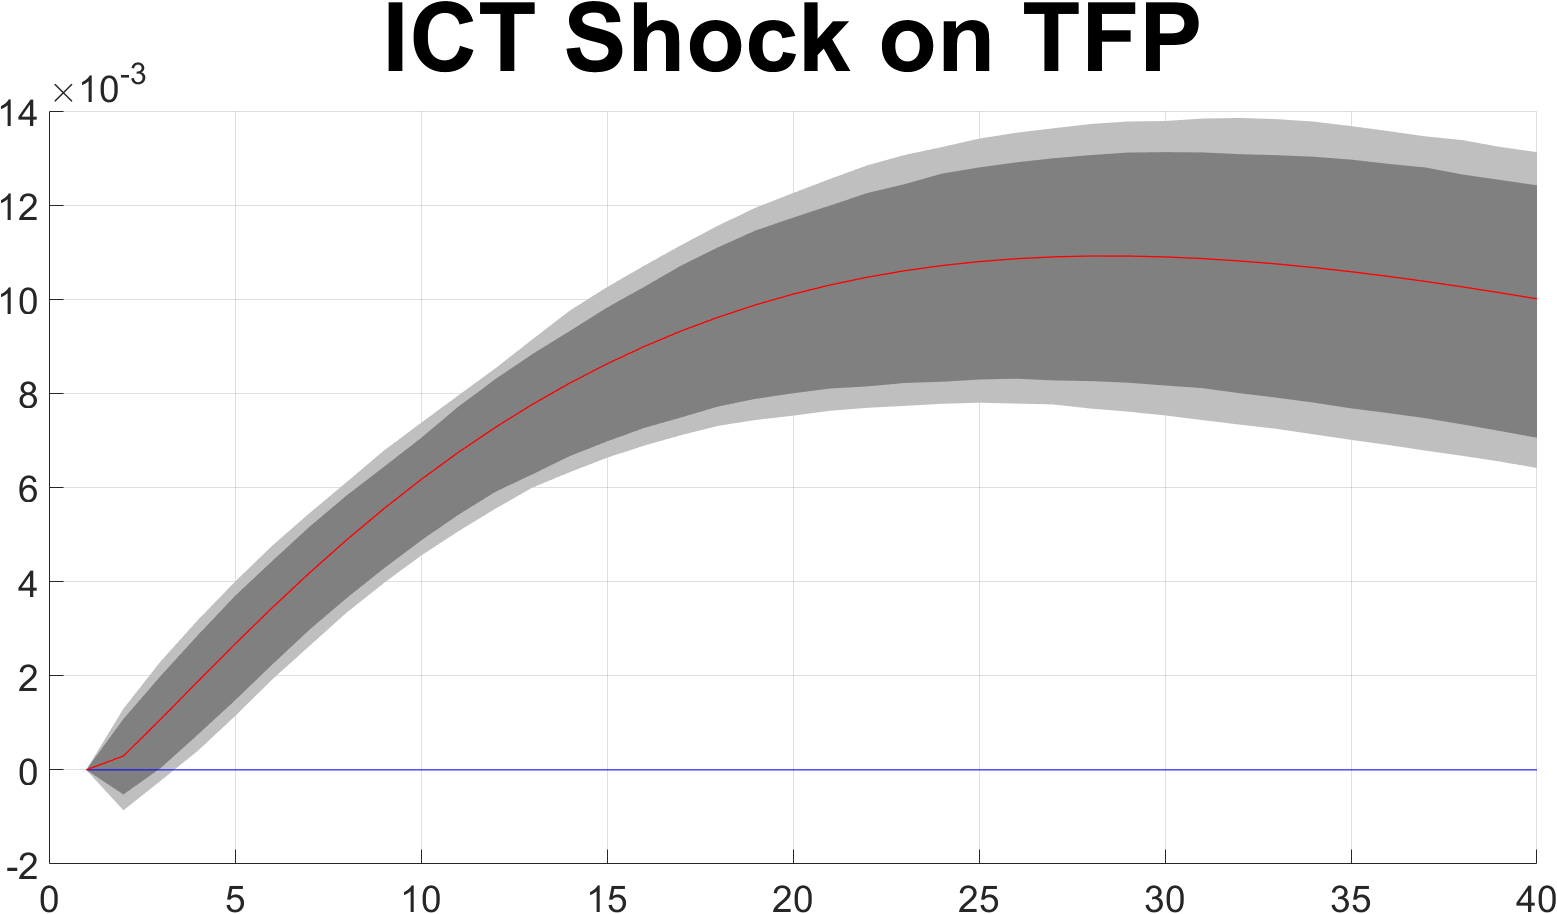
\includegraphics[scale=0.35]{MainFigures/fig_ICT_Shock_on_TFP_empirical_noH}
		\caption{Empirical impulse response of TFP to an ICT shock. The red solid lines are the estimated impulse responses to our ICT shock. The shaded dark gray area and the shaded light gray area are the $90$\% and $95$\% confidence intervals, respectively, from 2000 bias-corrected bootstrap replications of the reduced-form VAR. The horizontal axes refer to forecast horizon and the units of the vertical axes are percentage deviations.}
		\label{fig:TFP_main}
	\end{center}
\end{figure}

\newpage




	\begin{figure}[h!]
		\begin{center}
		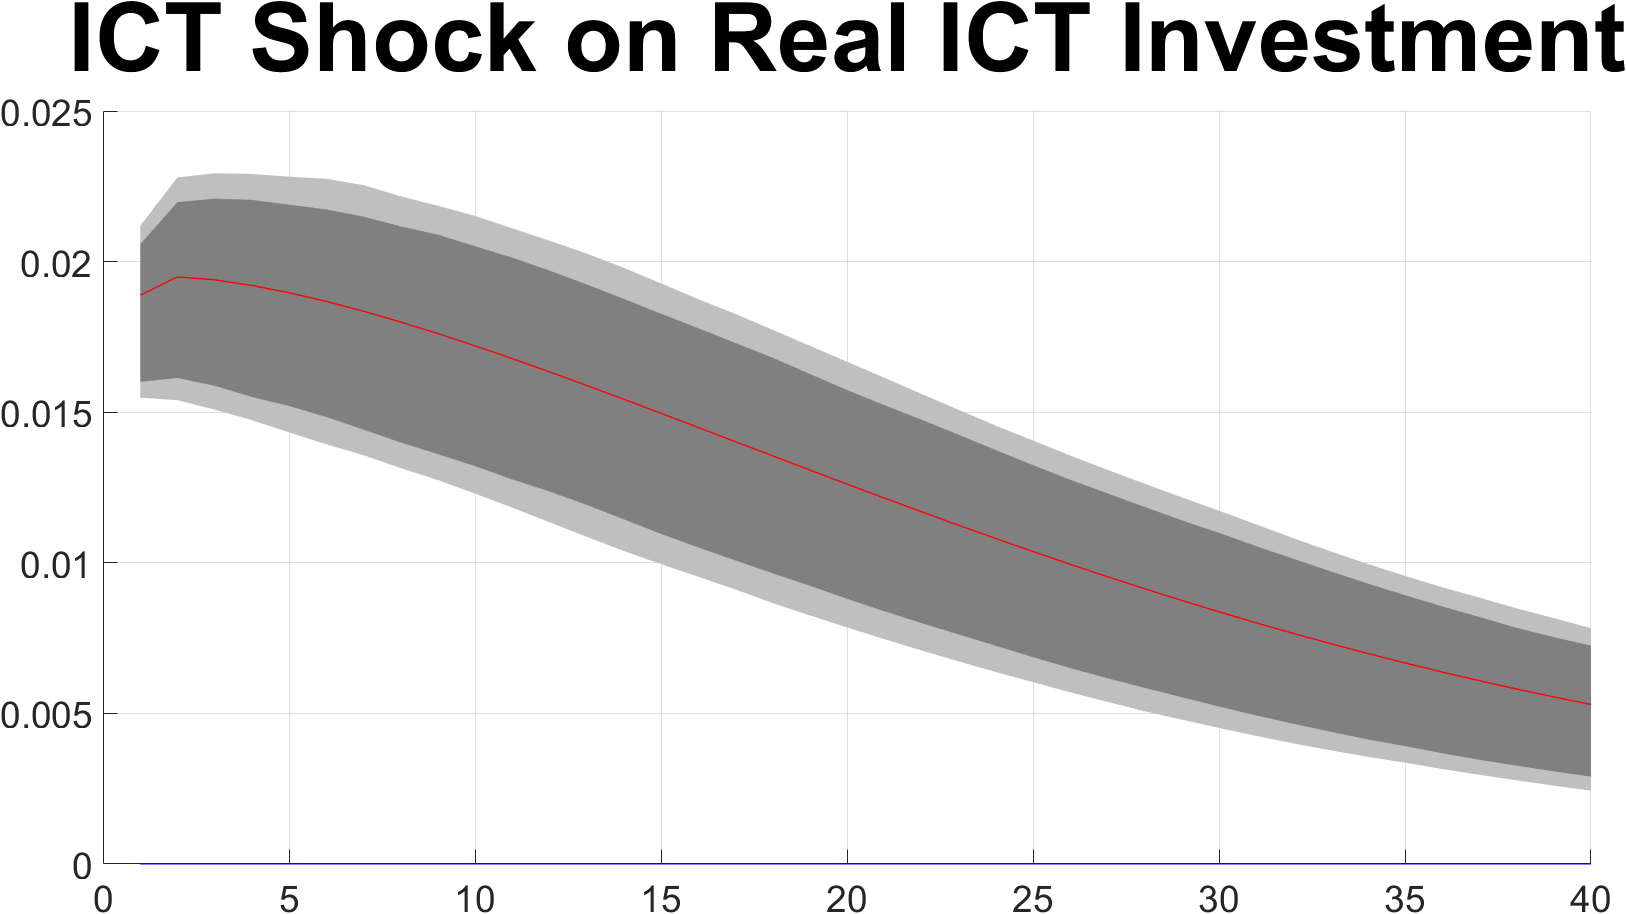
\includegraphics[scale=0.35]{MainFigures/fig_ICT_Shock_on_Real_ICT_Investment_empirical_noH}
		\caption{Empirical impulse response of real ICT investment to an ICT shock. The red solid lines are the estimated impulse responses to our ICT shock. The shaded dark gray area and the shaded light gray area are the $90$\% and $95$\% confidence intervals, respectively, from 2000 bias-corrected bootstrap replications of the reduced-form VAR. The horizontal axes refer to forecast horizon and the units of the vertical axes are percentage deviations.}
		\label{fig:ICT_main}
	\end{center} 
	\end{figure}

\newpage


	\begin{figure}[h!]
	\begin{center}
		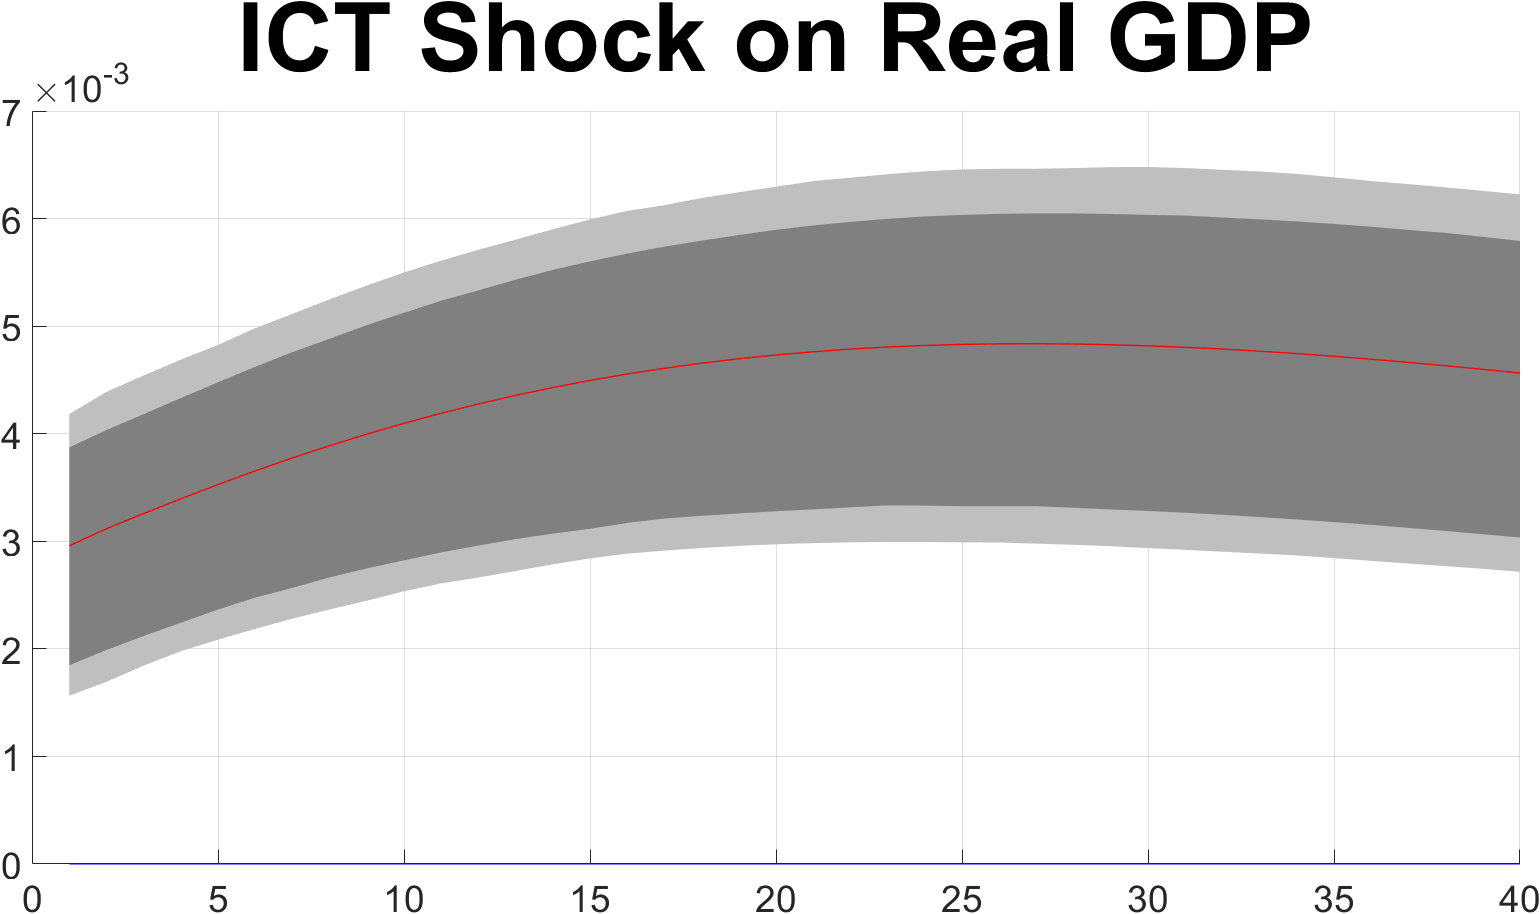
\includegraphics[scale=0.35]{MainFigures/fig_ICT_Shock_on_Real_GDP_empirical_noH}
		\caption{Empirical impulse response of real Gross Domestic Product to an ICT shock. The red solid lines are the estimated impulse responses to our ICT shock. The shaded dark gray area and the shaded light gray area are the $90$\% and $95$\% confidence intervals, respectively, from 2000 bias-corrected bootstrap replications of the reduced-form VAR. The horizontal axes refer to forecast horizon and the units of the vertical axes are percentage deviations.}
		\label{fig:GDP_main}
	\end{center} 
\end{figure}

\newpage


	\begin{figure}[h!]
	\begin{center}
		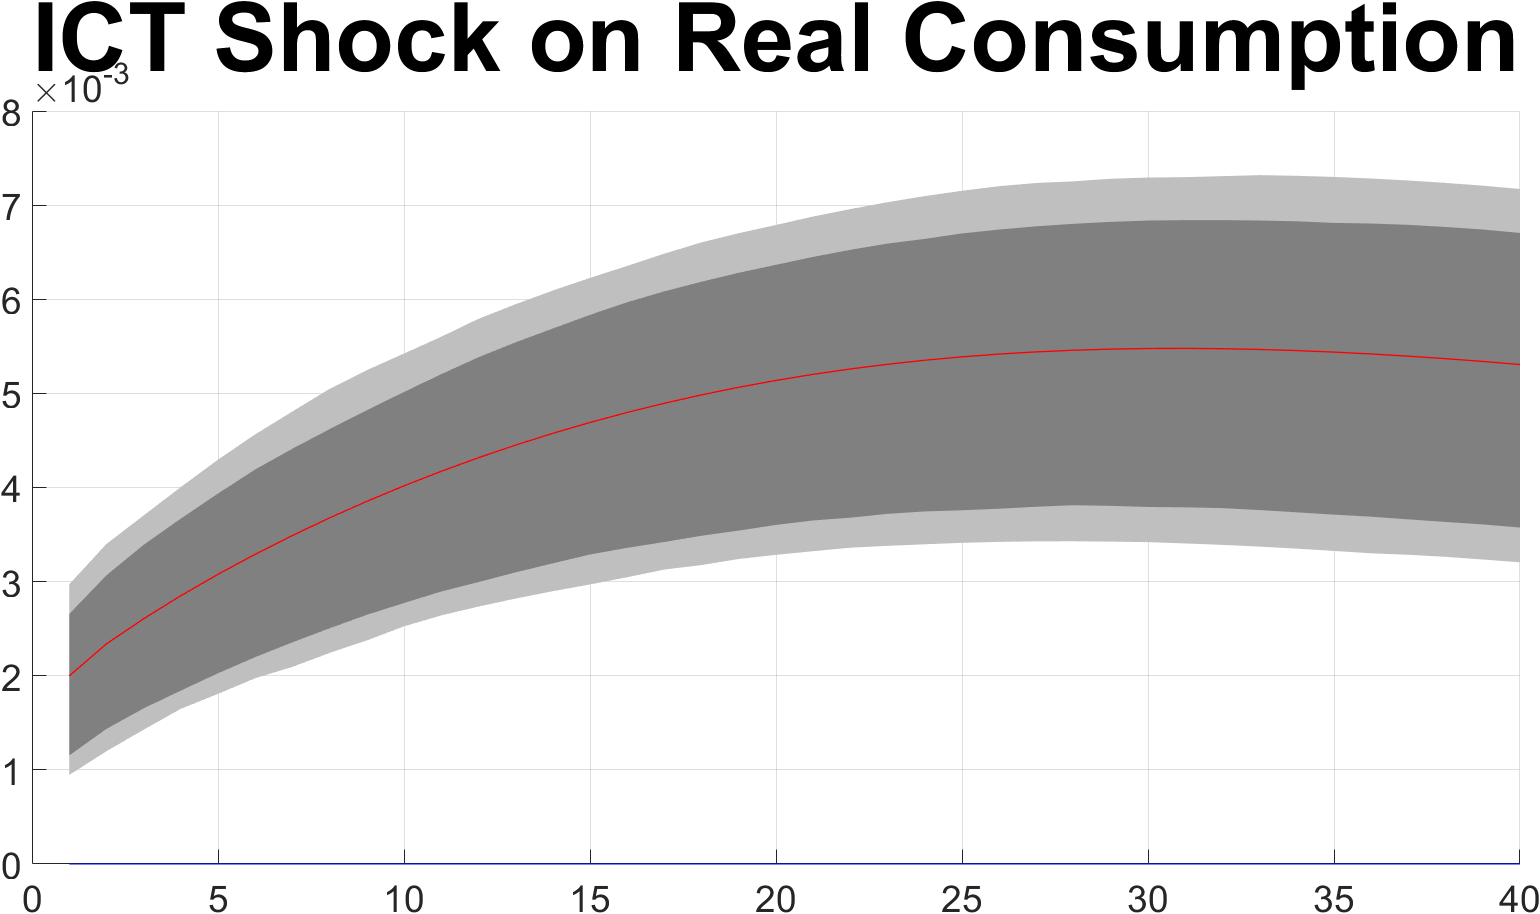
\includegraphics[scale=0.35]{MainFigures/fig_ICT_Shock_on_Real_Consumption_empirical_noH}
		\caption{Empirical impulse response of real consumption to an ICT shock. The red solid lines are the estimated impulse responses to our ICT shock. The shaded dark gray area and the shaded light gray area are the $90$\% and $95$\% confidence intervals, respectively, from 2000 bias-corrected bootstrap replications of the reduced-form VAR. The horizontal axes refer to forecast horizon and the units of the vertical axes are percentage deviations.}
		\label{fig:C_main}
	\end{center} 
\end{figure}

\newpage


	\begin{figure}[h!]
	\begin{center}
		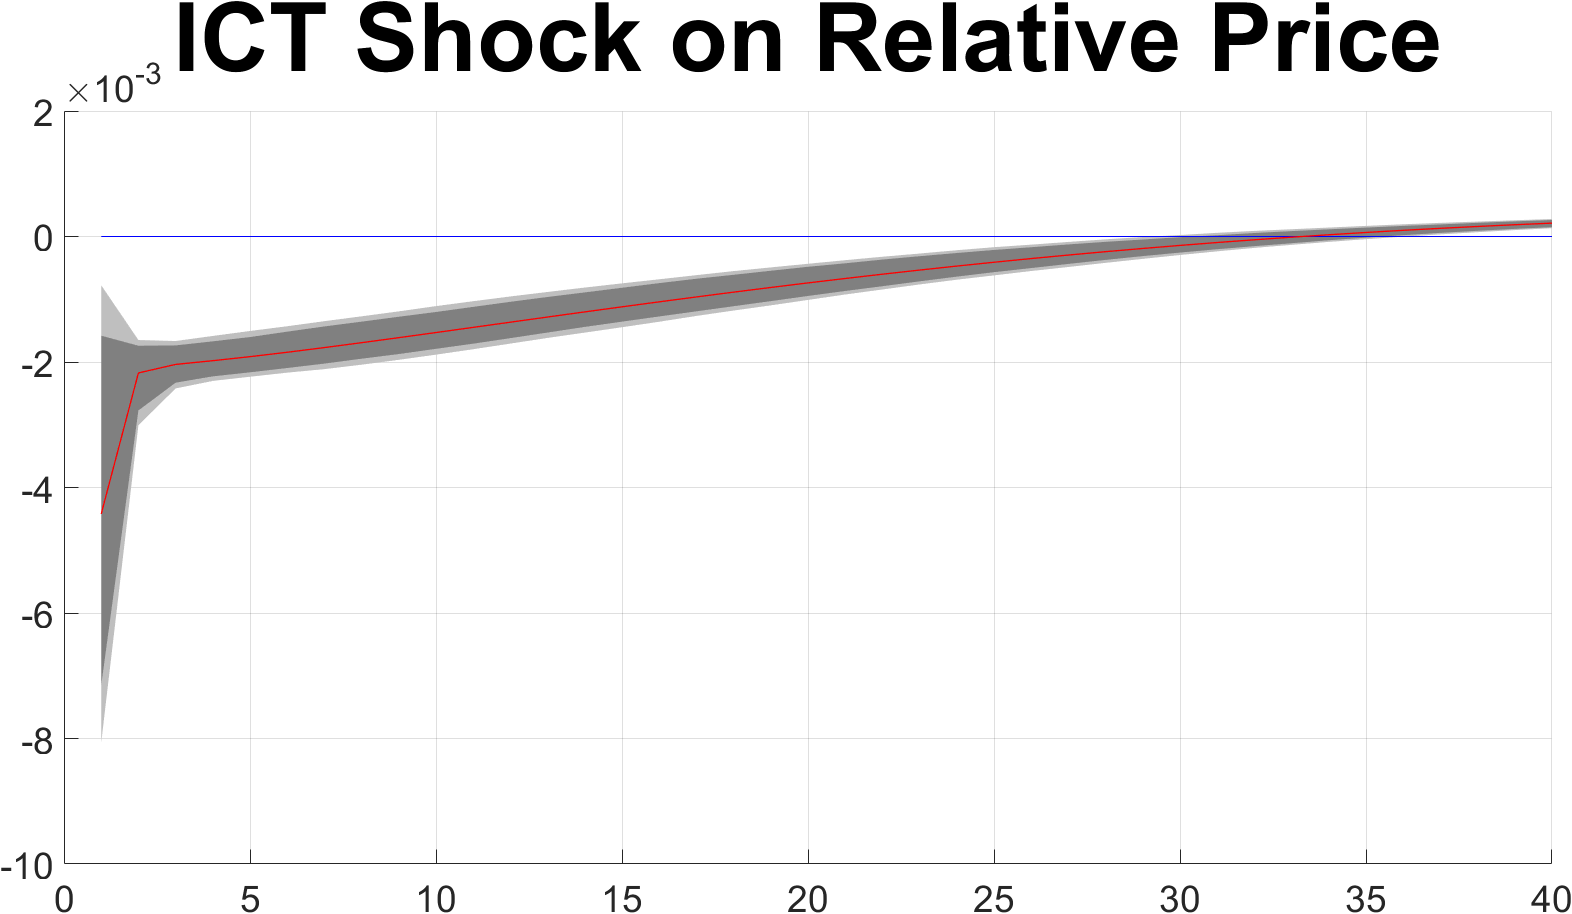
\includegraphics[scale=0.35]{MainFigures/fig_ICT_Shock_on_Relative_Price_empirical_noH}
		\caption{Empirical impulse response of relative price to an ICT shock. The red solid lines are the estimated impulse responses to our ICT shock. The shaded dark gray area and the shaded light gray area are the $90$\% and $95$\% confidence intervals, respectively, from 2000 bias-corrected bootstrap replications of the reduced-form VAR. The horizontal axes refer to forecast horizon and the units of the vertical axes are percentage deviations.}
		\label{fig:RP_main}
	\end{center} 
\end{figure}




\newpage

 
 
 \section{Variance Decomposition}\label{section:vardec}

 
 
 	\begin{table}[h!]
 		\begin{center}
 \begin{tabular}{lcccccccccc}
\hline
 	& $h = 1$ & $h = 4$ & $h = 8$ & $h = 16$ & $h = 24$ & $h = 40$ \\
 	\hline
TFP &  0       &  0.0023  &  0.0194 &   0.1088 &   0.2273  &  0.3382 \\
ICT Investment &  0.9997  &  0.9038  &  0.7964 &   0.6320 &   0.5310  &  0.4371 \\
Real GDP &  0.2620  &  0.3061  &  0.3486 &   0.3936 &   0.4046  &  0.3881 \\
Real Consumption &  0.1952  &  0.2638  &  0.3219 &   0.3931 &   0.4188  &  0.4064 \\
Relative Prices &  0.0618  &  0.0967  &  0.1276 &   0.1511 &   0.1516  &  0.1467 \\	
\hline
 	\end{tabular}
  		\caption{The letter $h$ denotes the forecast horizon. The numbers refer to the fraction of the forecast error variance of each variable at various forecast horizons to the identified ICT shock}
  \label{table:vardec}
  \end{center}
 \end{table}

\newpage

 \section{Removing Forward-Looking Variables}\label{section:removing_FL_Var}
 
 
 	\begin{figure}[h!]
 	\begin{center}
 		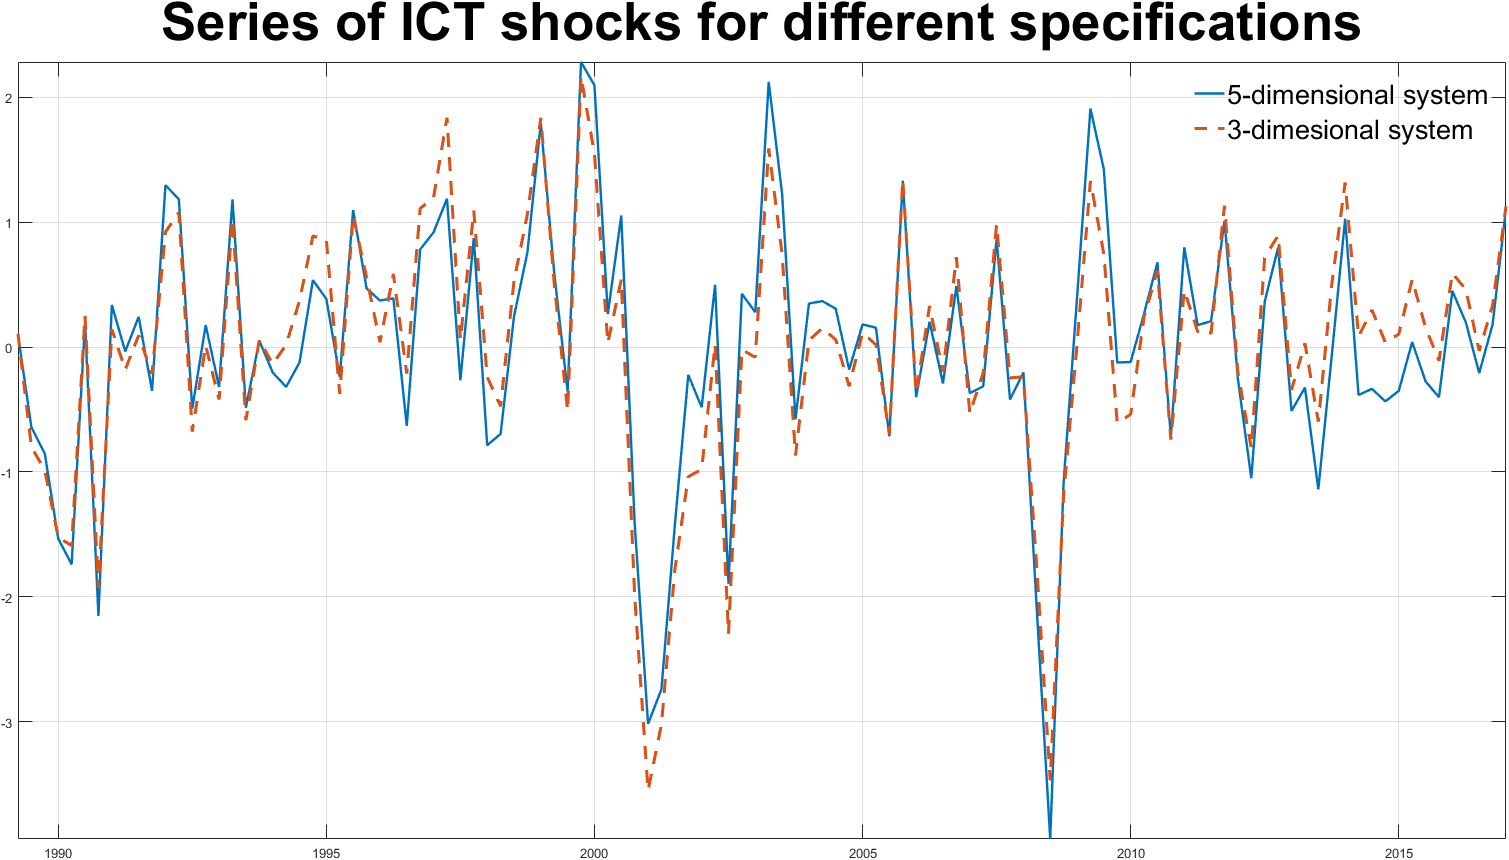
\includegraphics[scale=0.35]{MainFigures/Removing_FLVariables}
 		\caption{ICT shock series using the empirical strategy presented in \ref{section:empiricalstrategy_simple}. Blue solid line represents shock series for the 5-dimension system \ref{eq:mainSpecification} presented in \ref{section:mainSpec}. Red dotted line represents shock series for the 3-dimensional system presented in \ref{section:removing_FL_Var}.}
 		\label{fig:shockSeries_removing}
 	\end{center} 
 \end{figure}

\newpage

\section{Proof of Proposition \ref{prop:priceRestriction}}\label{section:proofpriceRestriction}

Notice that in this proof we use the same assumptions and the same notation in the 2-sector model presented in Section \ref{section:theory}.

\

First order condition with respect to labor input for firm $j$ is
\begin{eqnarray}\label{equation:FOC_j_l}
w_t =  (1 - a - b) p_t \eta_t \theta^c (k^i_t)^{\gamma} \bigg( \frac{k_t^c(j)}{l_t(j)} \bigg)^a \bigg( \frac{k_t^i(j)}{l_t(j)} \bigg)^b,
\end{eqnarray}
and first order condition with respect to labor input for firm $q$ is
\begin{eqnarray}\label{equation:FOC_q_l}
w_t = (1 - a - b) \eta_t \theta^c (k^i_t)^{\gamma} \bigg( \frac{k_t^c(q)}{l_t(q)} \bigg)^a \bigg( \frac{k_t^i(q)}{l_t(q)} \bigg)^b,
\end{eqnarray}
Since both production functions display identical input shares then in equilibrium input ratios must be the same over the two sectors, which is,
\begin{eqnarray}\label{eq:shares_result1}
\frac{k_t^c(j)}{l_t(j)} = \frac{k_t^c(q)}{l_t(q)},
\end{eqnarray}
\begin{eqnarray}\label{eq:shares_result2}
\frac{k_t^i(j)}{l_t(j)} = \frac{k_t^i(q)}{l_t(q)},
\end{eqnarray}
\begin{eqnarray*}\label{eq:shares_result3}
\frac{k_t^i(j)}{k^c_t(j)} = \frac{k_t^i(q)}{k^c_t(q)}.
\end{eqnarray*}
Now, dividing \ref{equation:FOC_j_l} over \ref{equation:FOC_q_l}, we can use \ref{eq:shares_result1} and \ref{eq:shares_result2} to obtain
\begin{eqnarray}\label{eq:result_proof}
1 = \frac{1}{p_t} \frac{\theta^c_t}{\theta^i_t} \ \ \Rightarrow \ \ p_t = \frac{\theta^c_t}{\theta^i_t}.
\end{eqnarray}
From Equation \ref{eq:result_proof}, it is clear that the equilibrium path of $p_t$ is fully independent on the past, current, and future values of neutral technology, $\eta_t$. 
\qed

\newpage

\section{Controlling for News Shocks - Two-Step Identification Strategy}

\subsection{Impulse Responses}\label{section:IRF_2step}

\begin{figure}[h!]
	\begin{subfigure}{.5\textwidth}
		\centering
		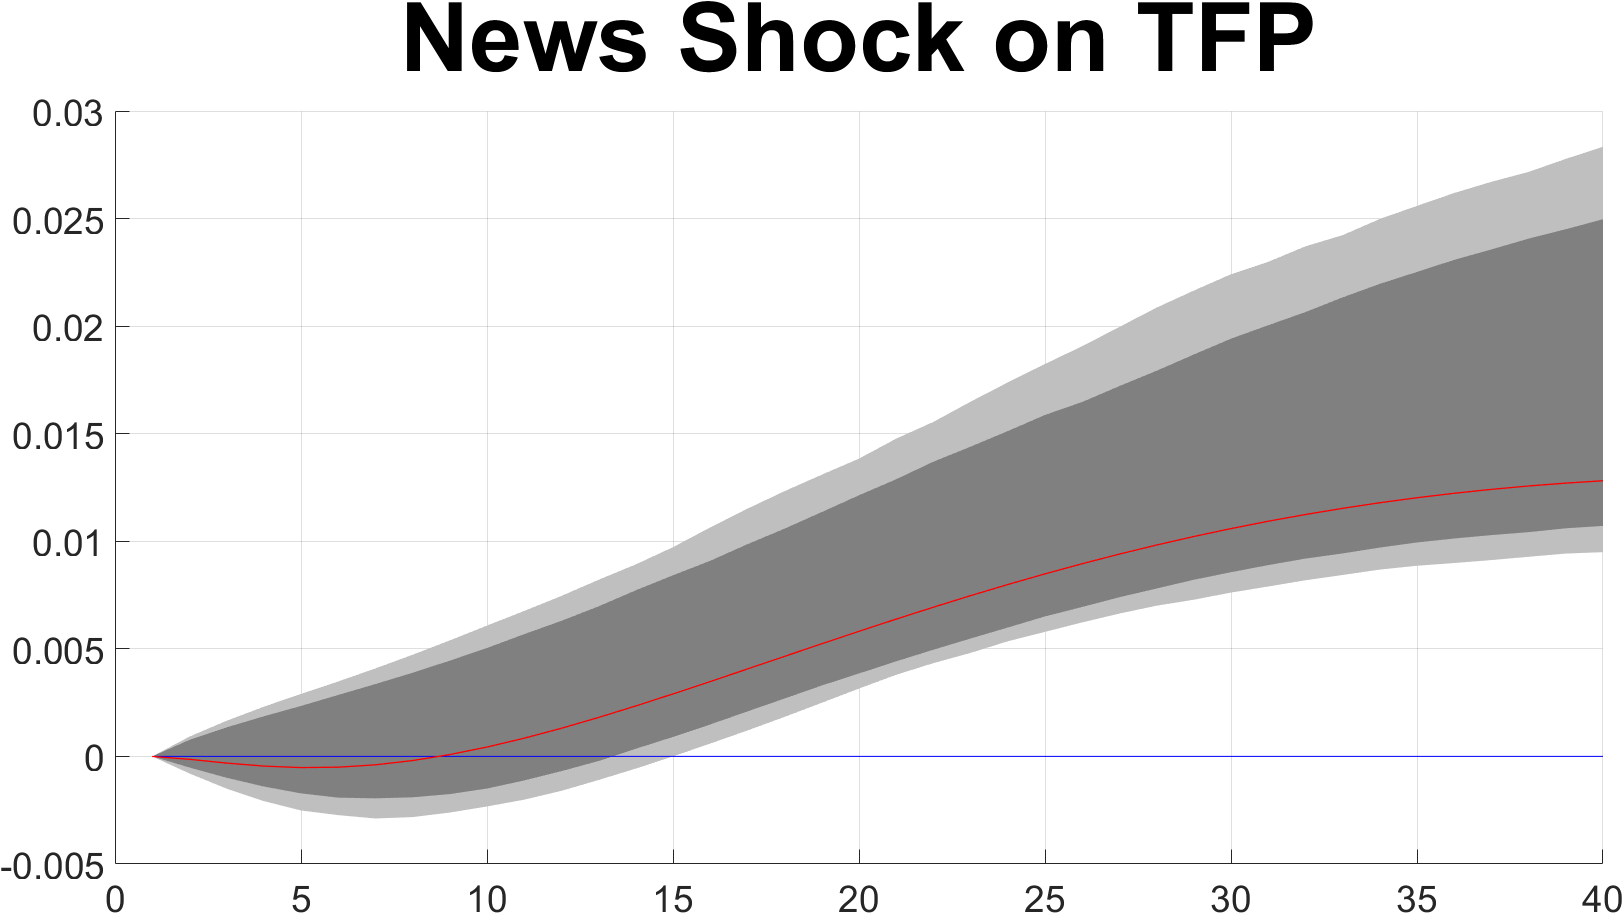
\includegraphics[width=1\linewidth]{MainFigures/fig_News_Shock_on_TFP__controllinNEWS_}
	\end{subfigure}%
	\begin{subfigure}{.5\textwidth}
		\centering
		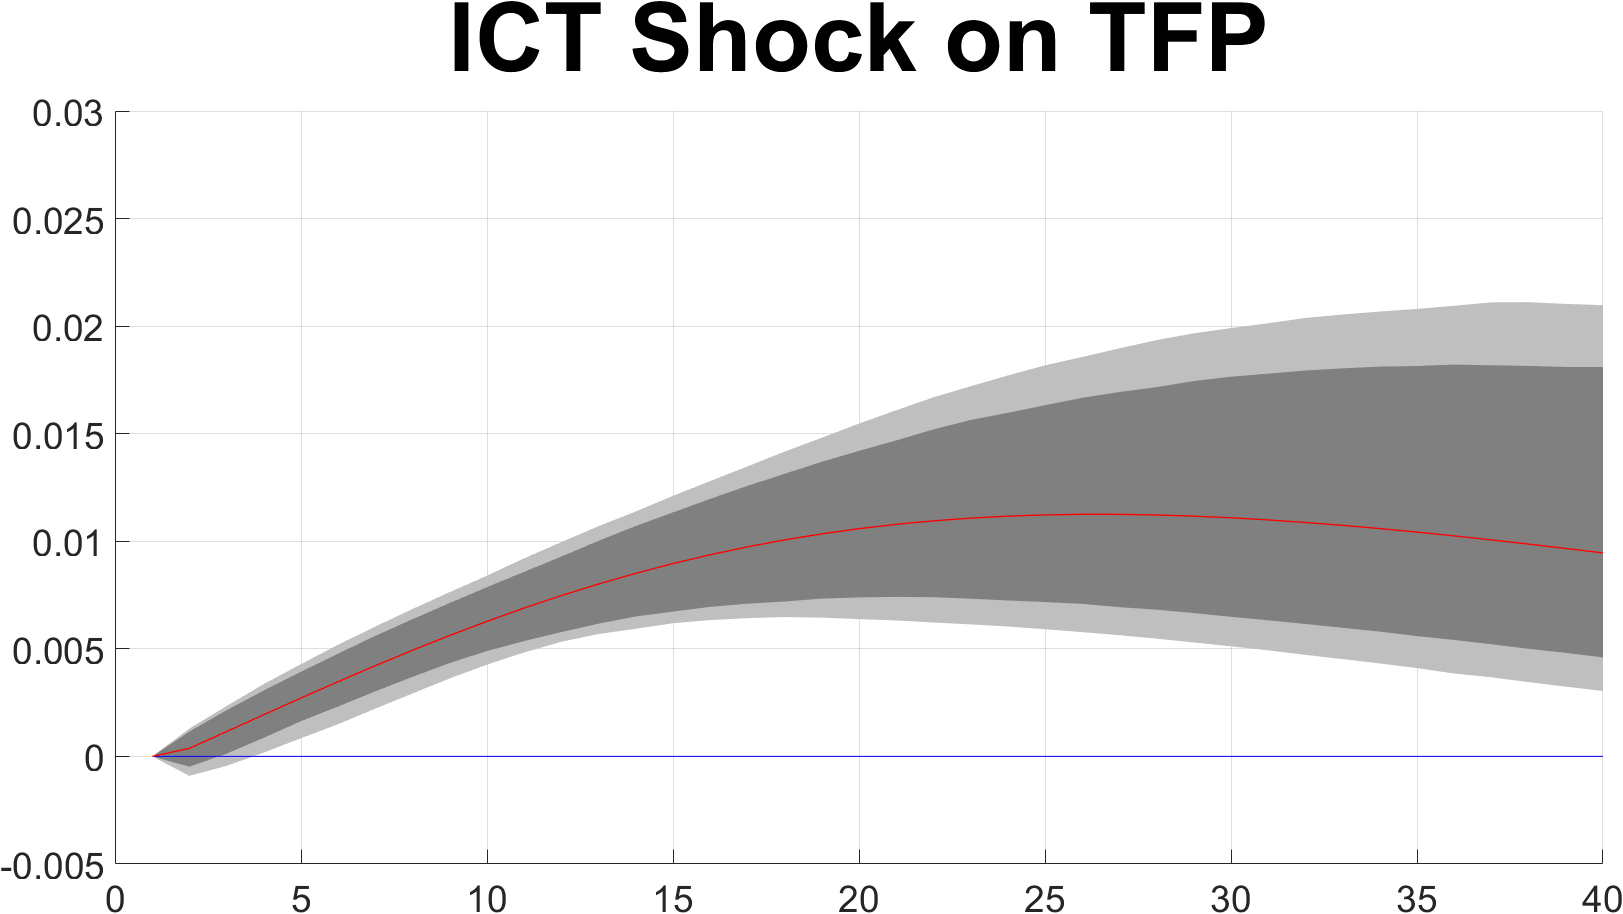
\includegraphics[width=1\linewidth]{MainFigures/fig_ICT_Shock_on_TFP__controllinNEWS_}
	\end{subfigure}
%%%%%%%%%%%%%%%%%%%%%%%%%%%%%%%%%%%%%%%%%%%%%%%%%%%%%%%%%%%%
\begin{subfigure}{.5\textwidth}
	\centering
	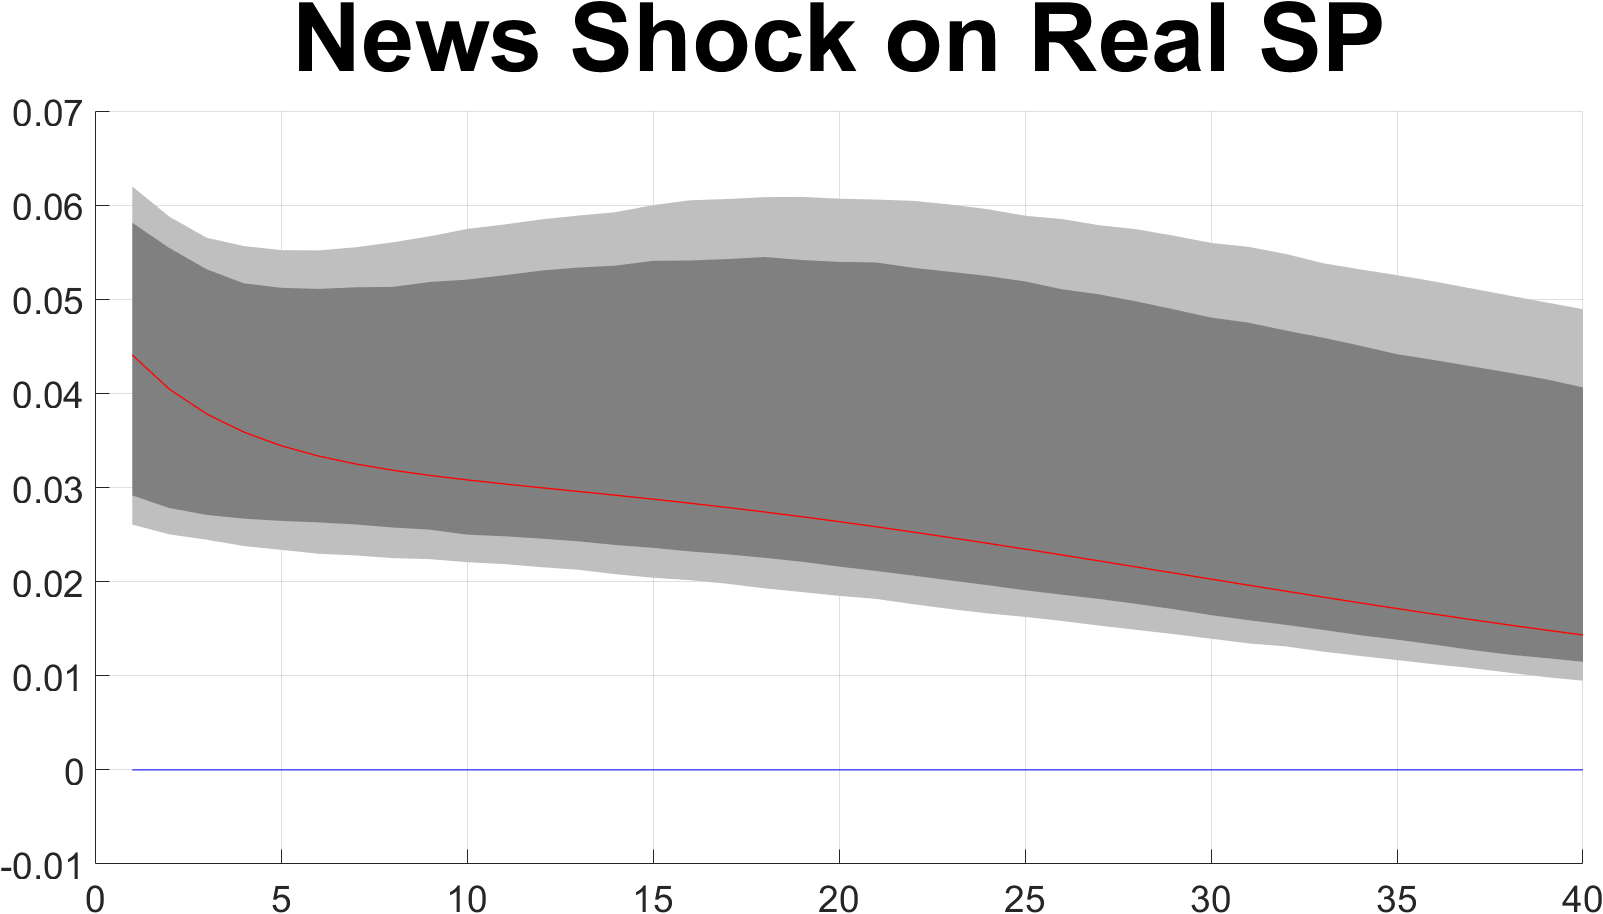
\includegraphics[width=1\linewidth]{MainFigures/fig_News_Shock_on_Real_SP__controllinNEWS_}
\end{subfigure}%
\begin{subfigure}{.5\textwidth}
	\centering
	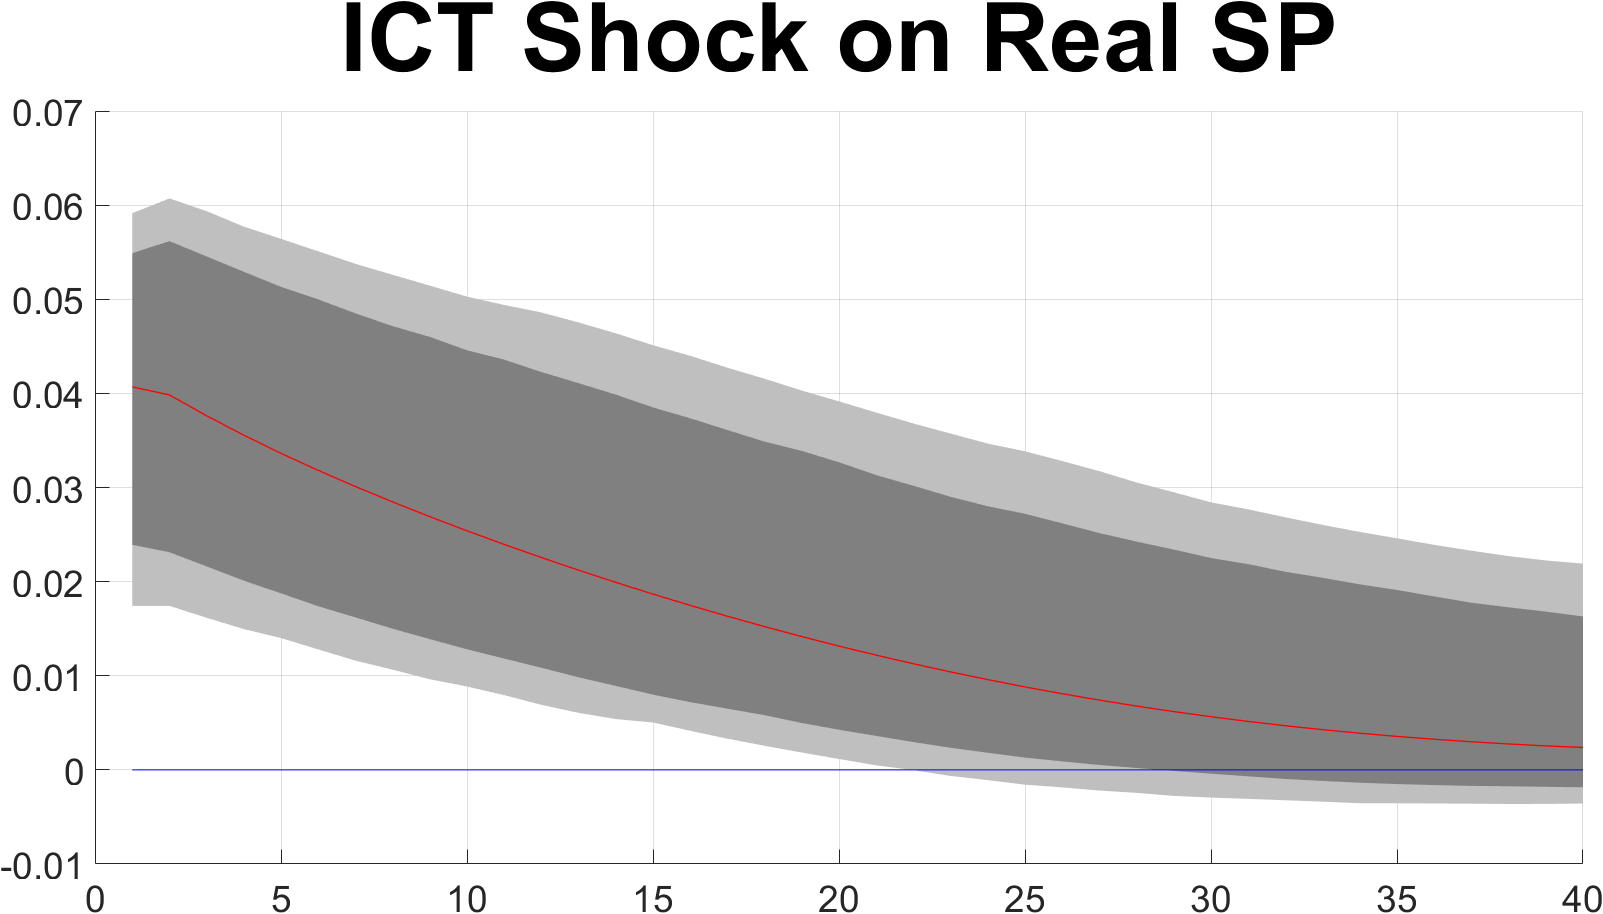
\includegraphics[width=1\linewidth]{MainFigures/fig_ICT_Shock_on_Real_SP__controllinNEWS_}
\end{subfigure}
%%%%%%%%%%%%%%%%%%%%%%%%%%%%%%%%%%%%%%%%%%%%%%%%%%%%%%%%%%%%
\begin{subfigure}{.5\textwidth}
	\centering
	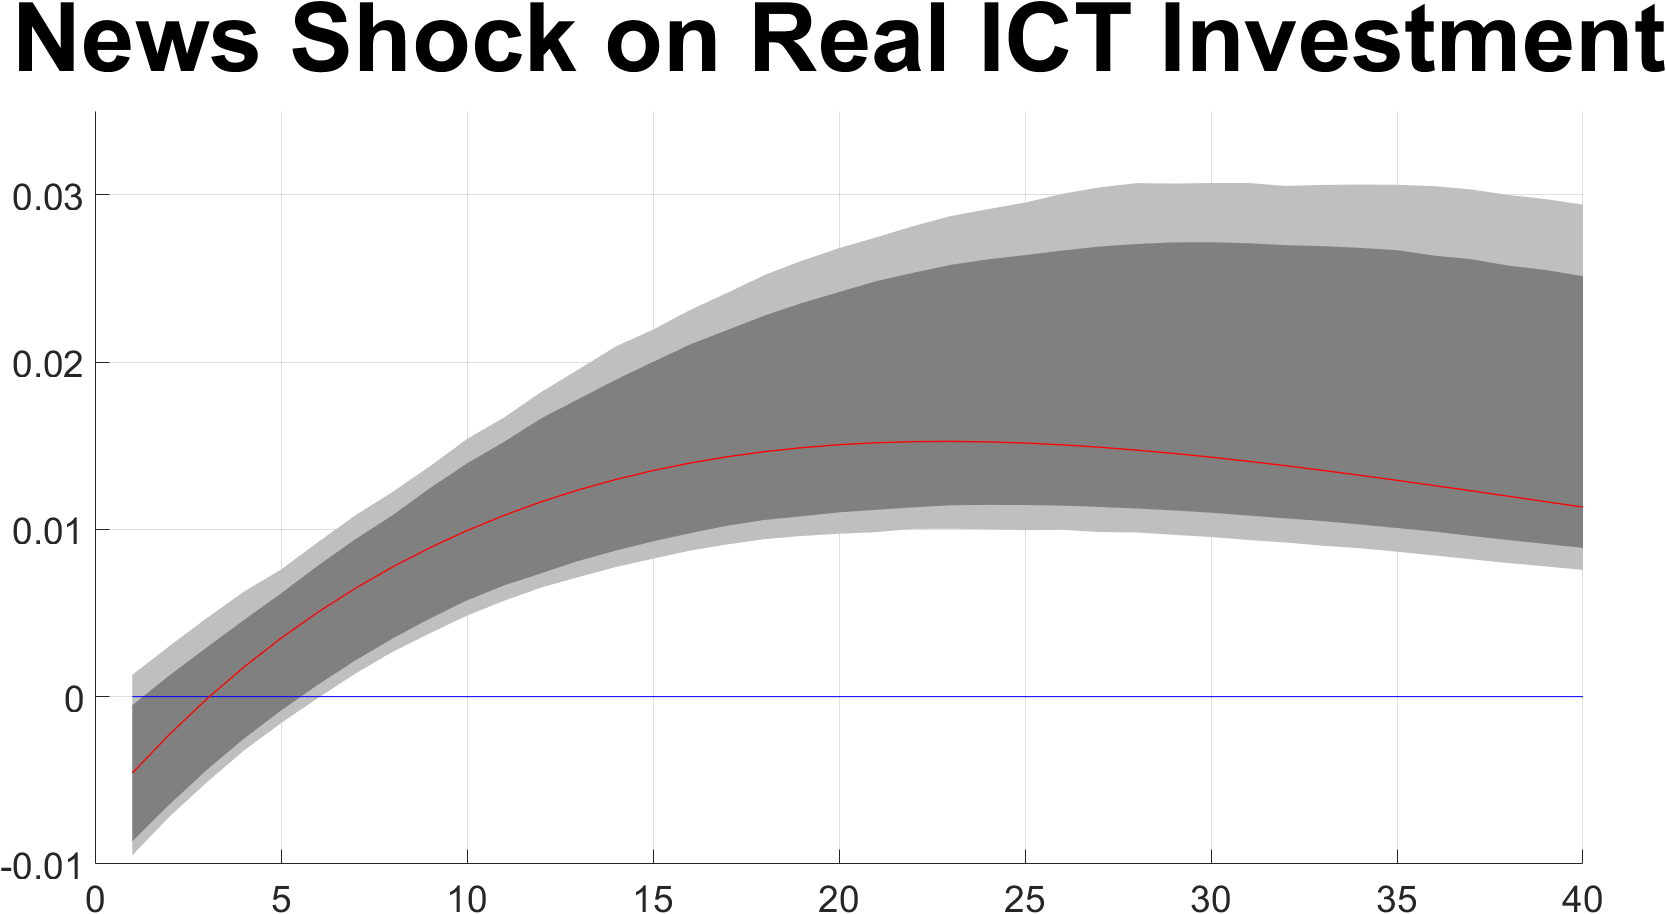
\includegraphics[width=1\linewidth]{MainFigures/fig_News_Shock_on_Real_ICT_Investment__controllinNEWS_}
\end{subfigure}%
\begin{subfigure}{.5\textwidth}
	\centering
	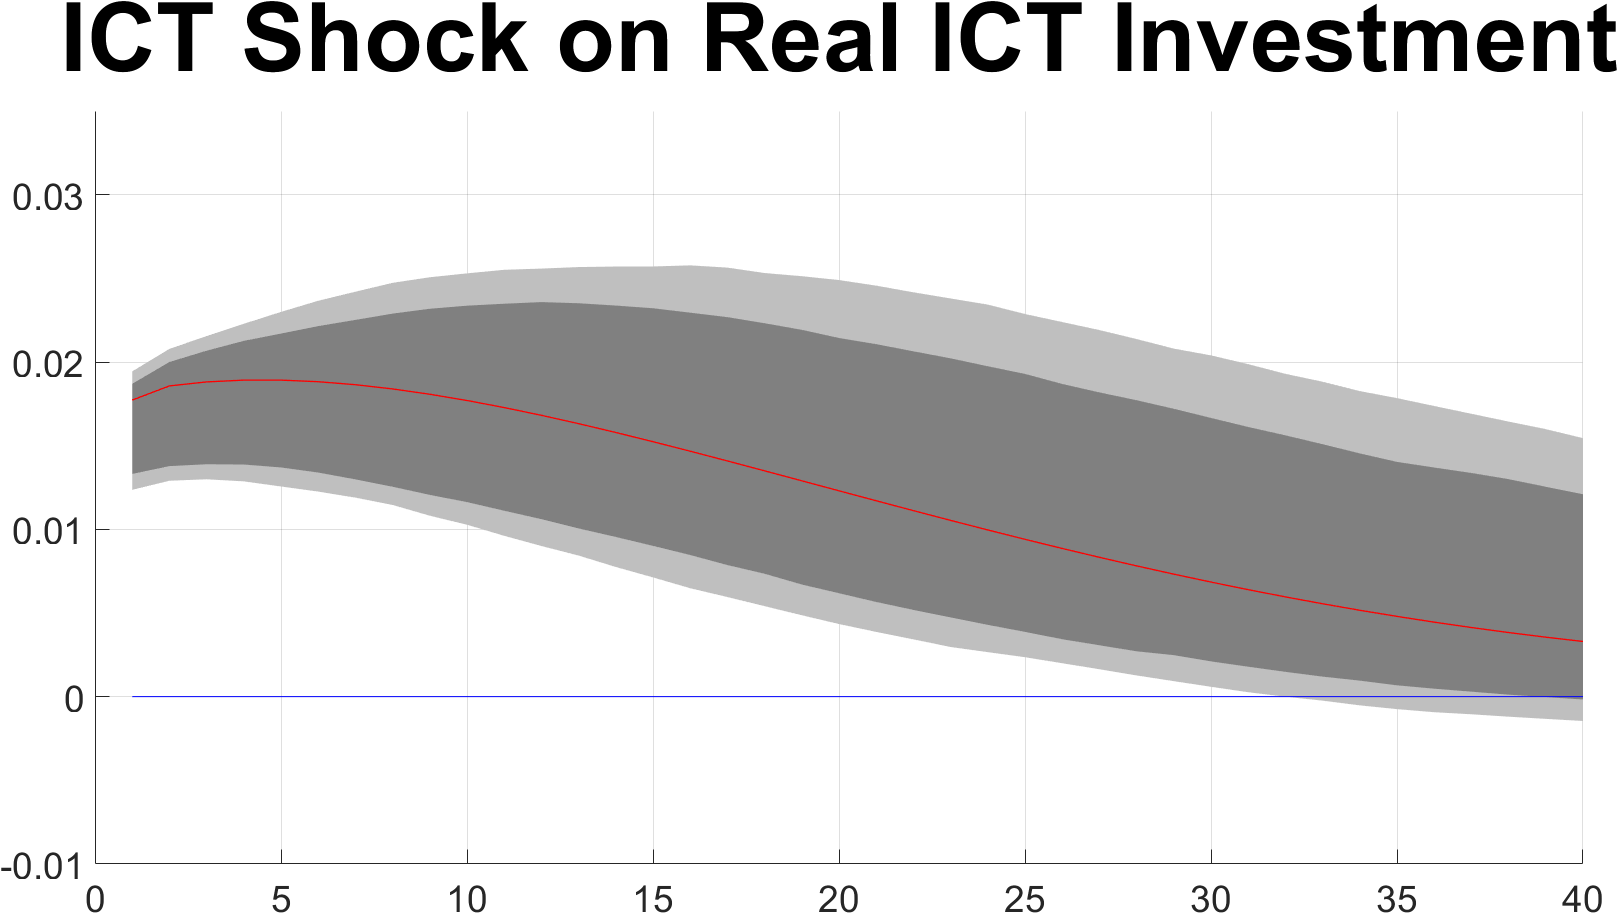
\includegraphics[width=1\linewidth]{MainFigures/fig_ICT_Shock_on_Real_ICT_Investment__controllinNEWS_}
\end{subfigure}
%%%%%%%%%%%%%%%%%%%%%%%%%%%%%%%%%%%%%%%%%%%%%%%%%%%%%%%%%%%%
	\caption{Empirical impulse responses of TFP, Real Stock Prices, and Real ICT Investment to a news shock and an ICT shock. The red solid lines are the estimated impulse responses to our ICT shock. The shaded dark gray area and the shaded light gray area are the $90$\% and $95$\% confidence intervals, respectively, from 2000 bias-corrected bootstrap replications of the reduced-form VAR. The horizontal axes refer to forecast horizon and the units of the vertical axes are percentage deviations.}
	\label{fig:2stepIRF_first}
\end{figure}

\newpage

\begin{figure}[h!]
\begin{subfigure}{.5\textwidth}
	\centering
	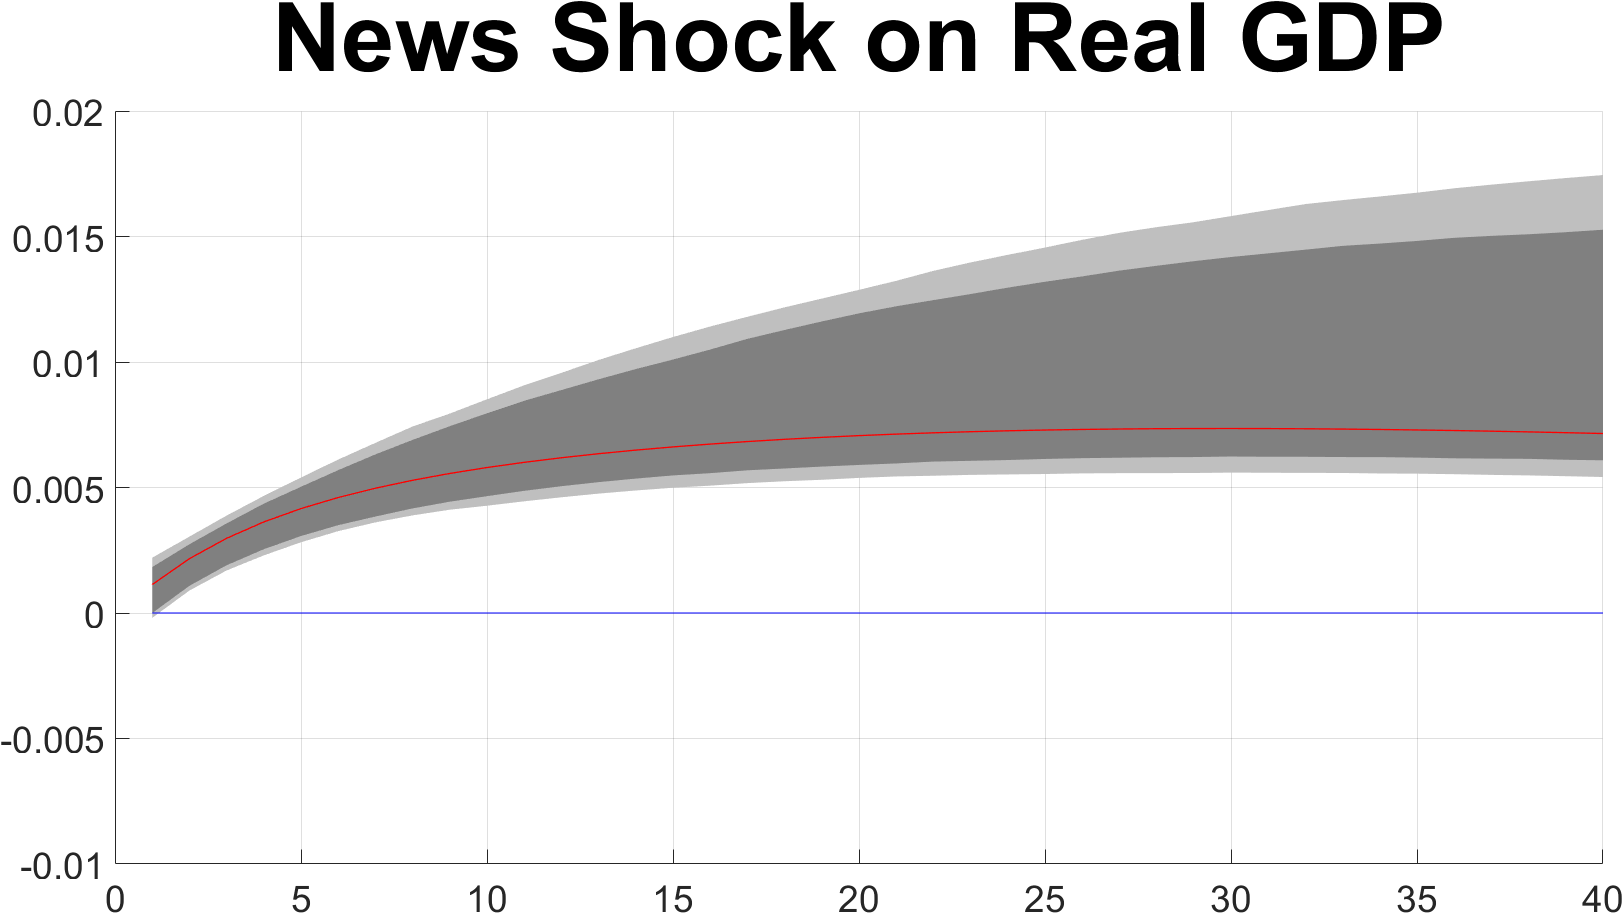
\includegraphics[width=1\linewidth]{MainFigures/fig_News_Shock_on_Real_GDP__controllinNEWS_}
\end{subfigure}%
\begin{subfigure}{.5\textwidth}
	\centering
	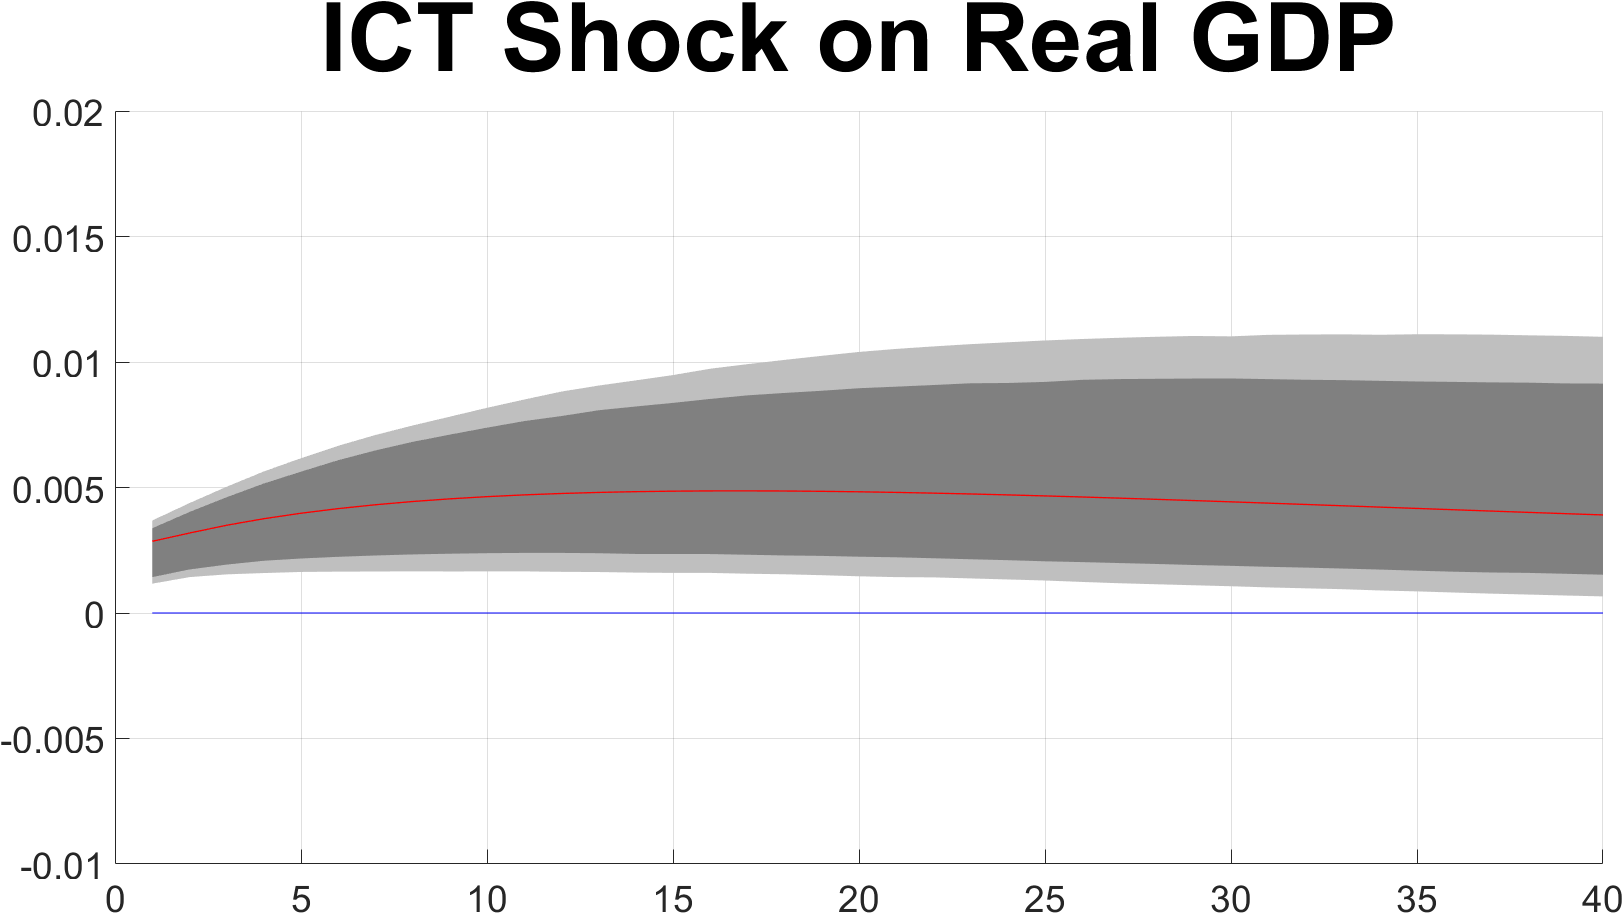
\includegraphics[width=1\linewidth]{MainFigures/fig_ICT_Shock_on_Real_GDP__controllinNEWS_}
\end{subfigure}
%%%%%%%%%%%%%%%%%%%%%%%%%%%%%%%%%%%%%%%%%%%%%%%%%%%%%%%%%%%%
\begin{subfigure}{.5\textwidth}
	\centering
	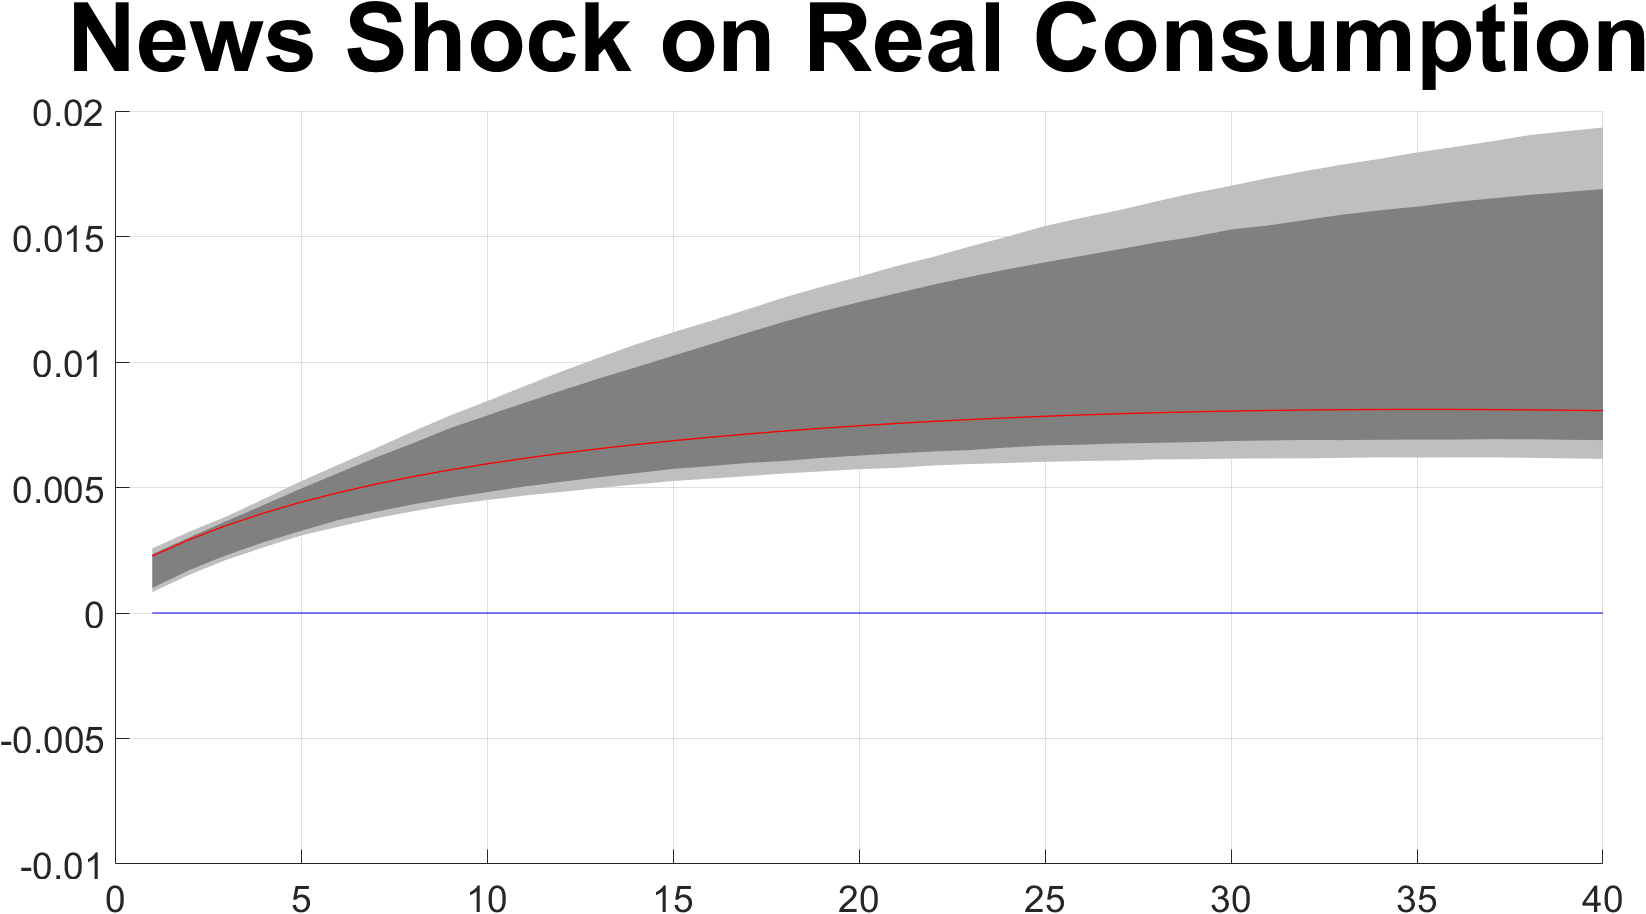
\includegraphics[width=1\linewidth]{MainFigures/fig_News_Shock_on_Real_Consumption__controllinNEWS_}
\end{subfigure}%
\begin{subfigure}{.5\textwidth}
	\centering
	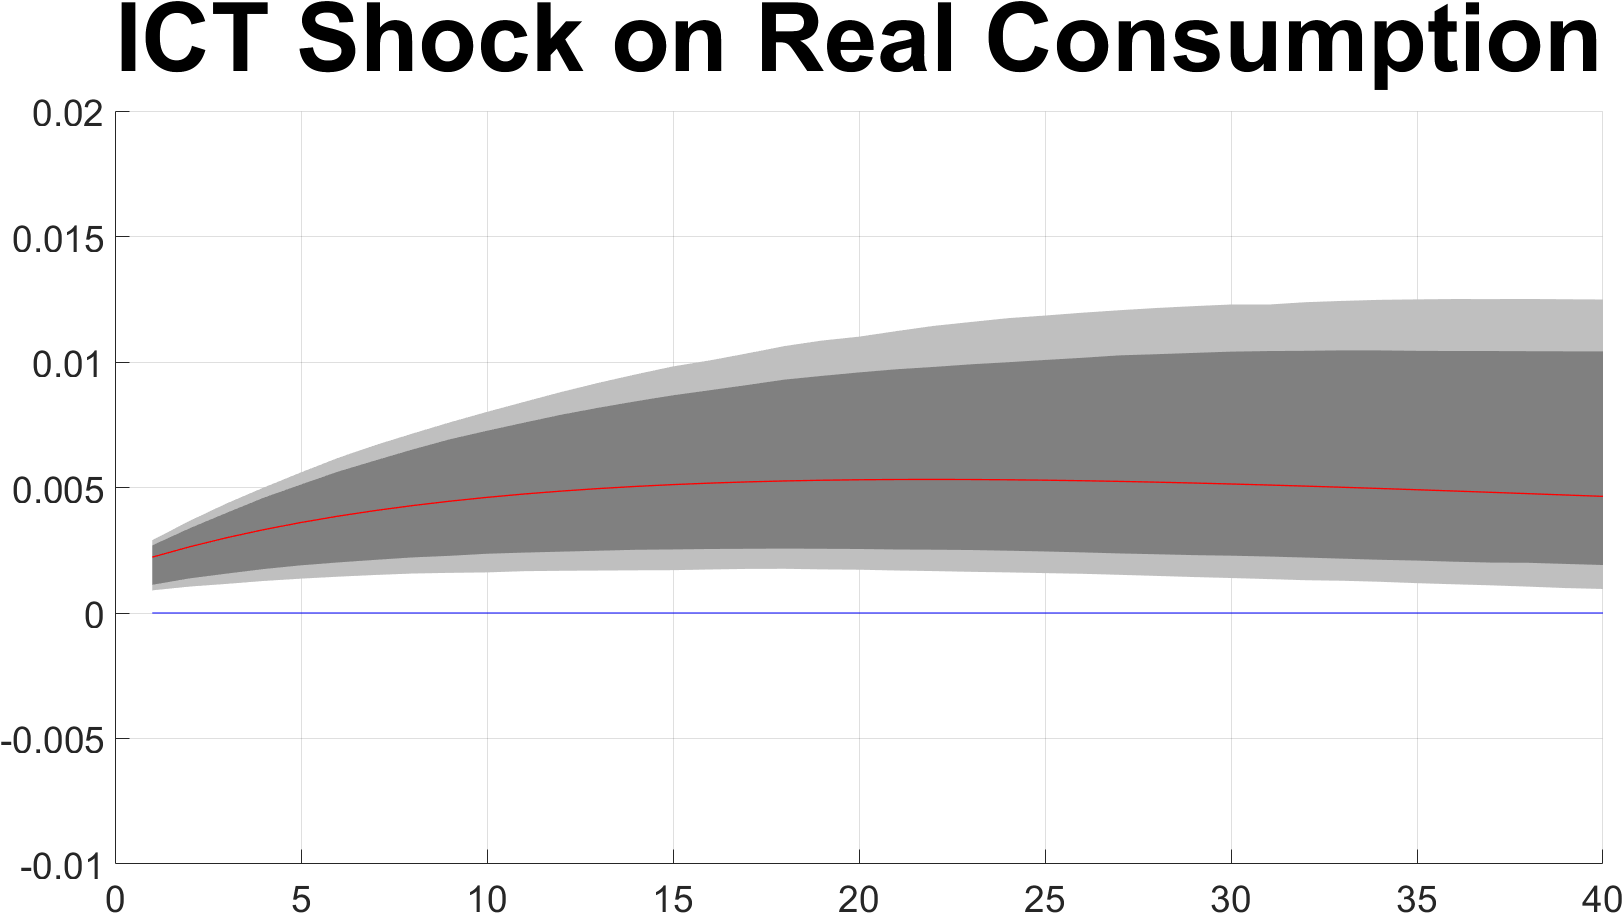
\includegraphics[width=1\linewidth]{MainFigures/fig_ICT_Shock_on_Real_Consumption__controllinNEWS_}
\end{subfigure}
%%%%%%%%%%%%%%%%%%%%%%%%%%%%%%%%%%%%%%%%%%%%%%%%%%%%%%%%%%%%
\begin{subfigure}{.5\textwidth}
	\centering
	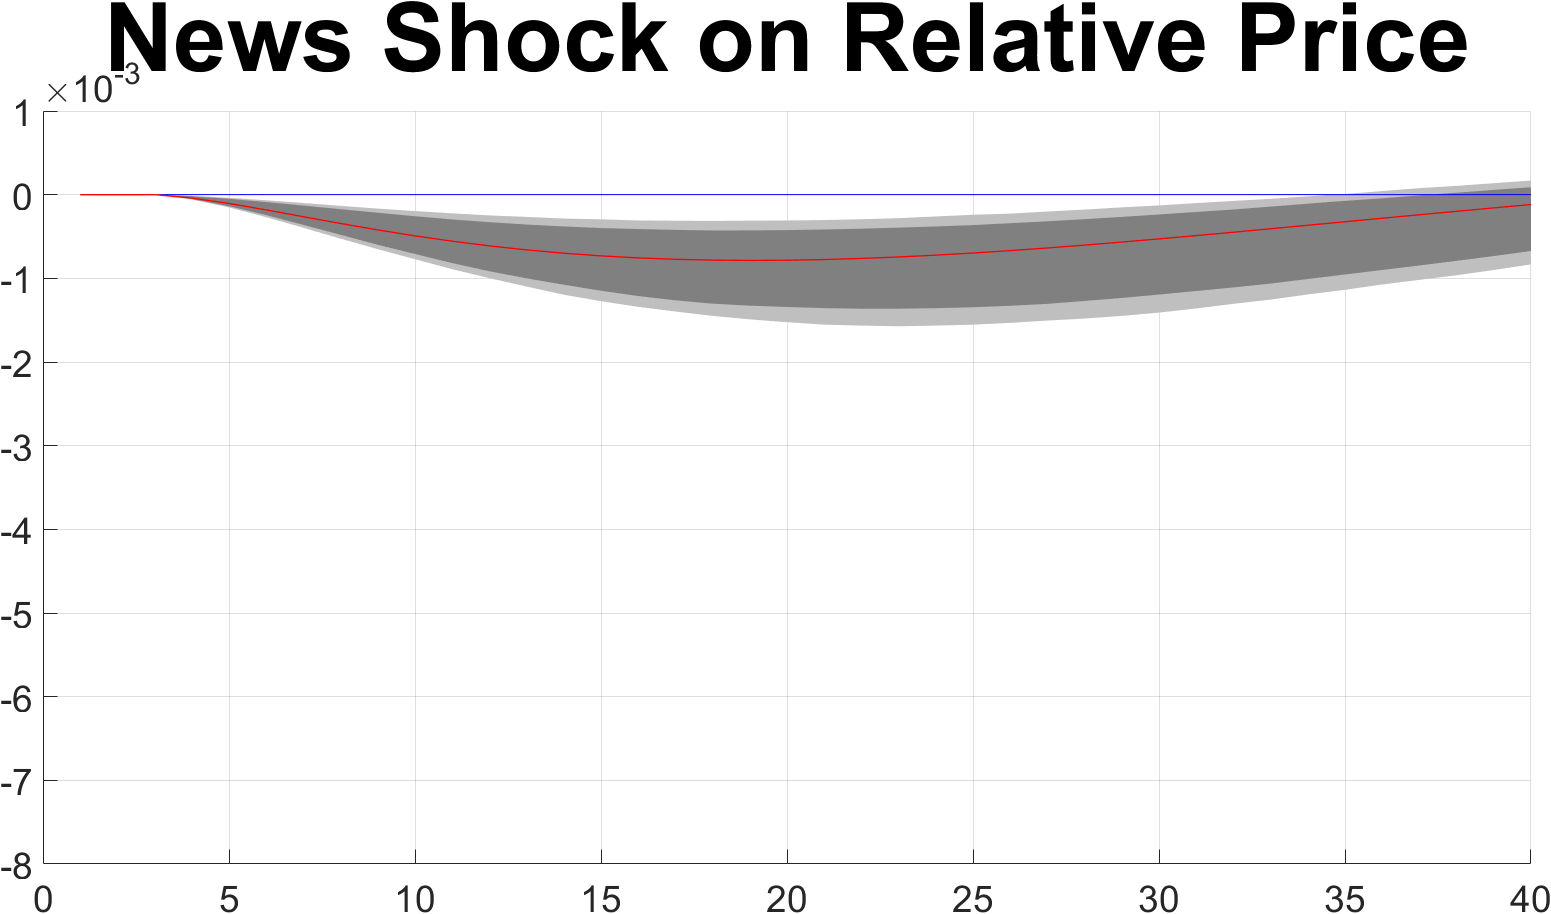
\includegraphics[width=1\linewidth]{MainFigures/fig_News_Shock_on_Relative_Price__controllinNEWS_}
\end{subfigure}%
\begin{subfigure}{.5\textwidth}
	\centering
	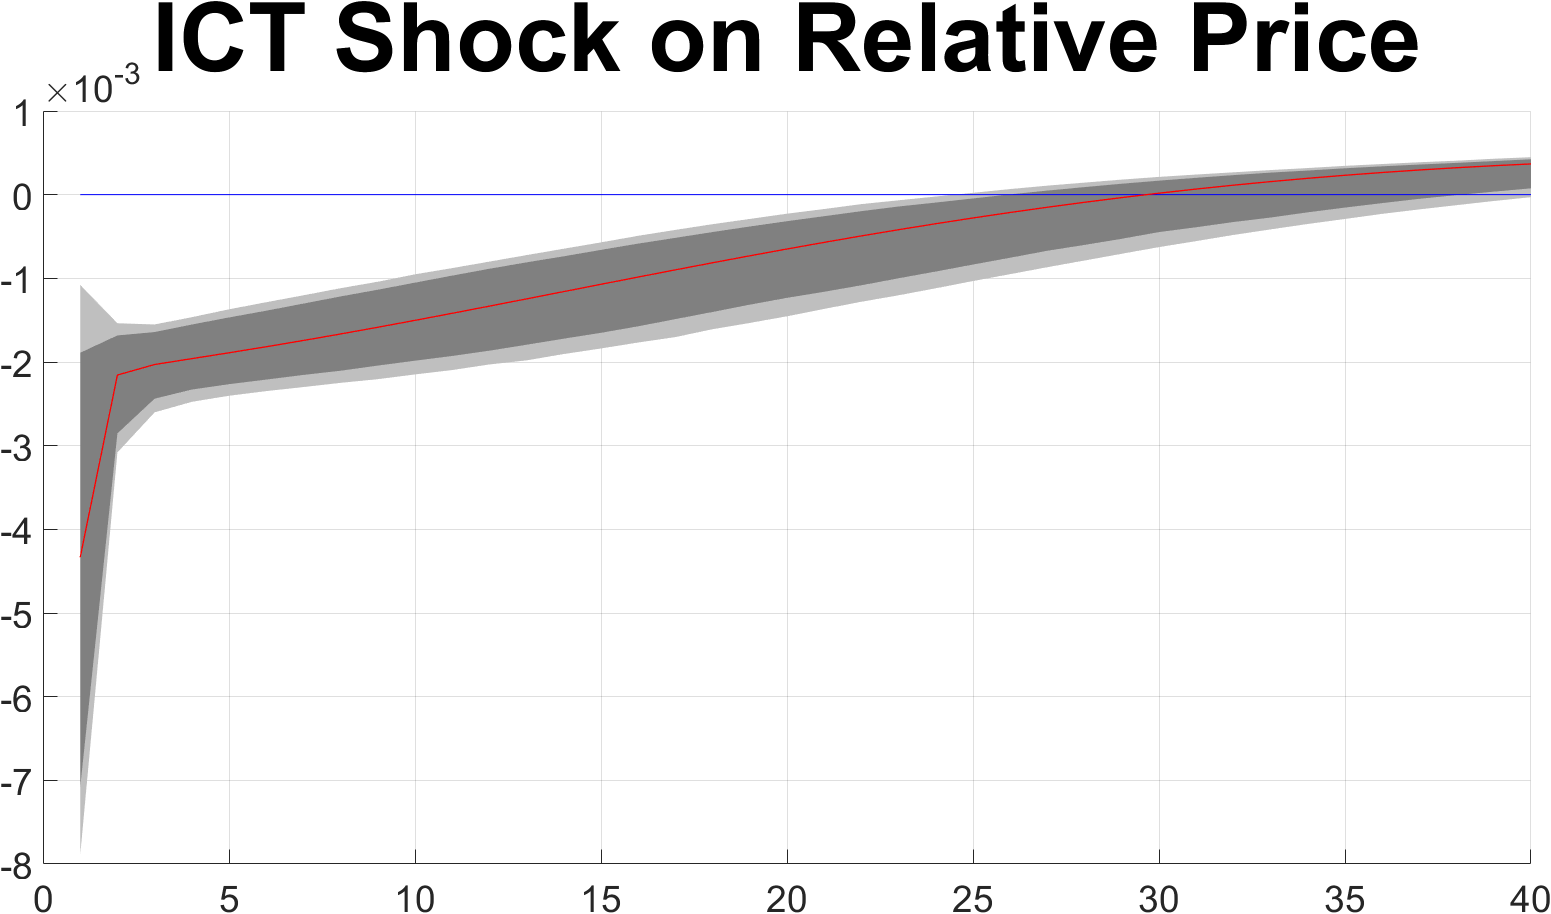
\includegraphics[width=1\linewidth]{MainFigures/fig_ICT_Shock_on_Relative_Price__controllinNEWS_}
\end{subfigure}
%%%%%%%%%%%%%%%%%%%%%%%%%%%%%%%%%%%%%%%%%%%%%%%%%%%%%%%%%%%%
	\caption{Empirical impulse responses of Real GDP, Real Consumption, and Relative Prices to a news shock and an ICT shock. The red solid lines are the estimated impulse responses to our ICT shock. The shaded dark gray area and the shaded light gray area are the $90$\% and $95$\% confidence intervals, respectively, from 2000 bias-corrected bootstrap replications of the reduced-form VAR. The horizontal axes refer to forecast horizon and the units of the vertical axes are percentage deviations.}
\label{fig:2stepIRF_second}
\end{figure}


\newpage


\subsection{ICT Shock Series}\label{section:ICTshockseries_2step}

 	\begin{figure}[h!]
	\begin{center}
		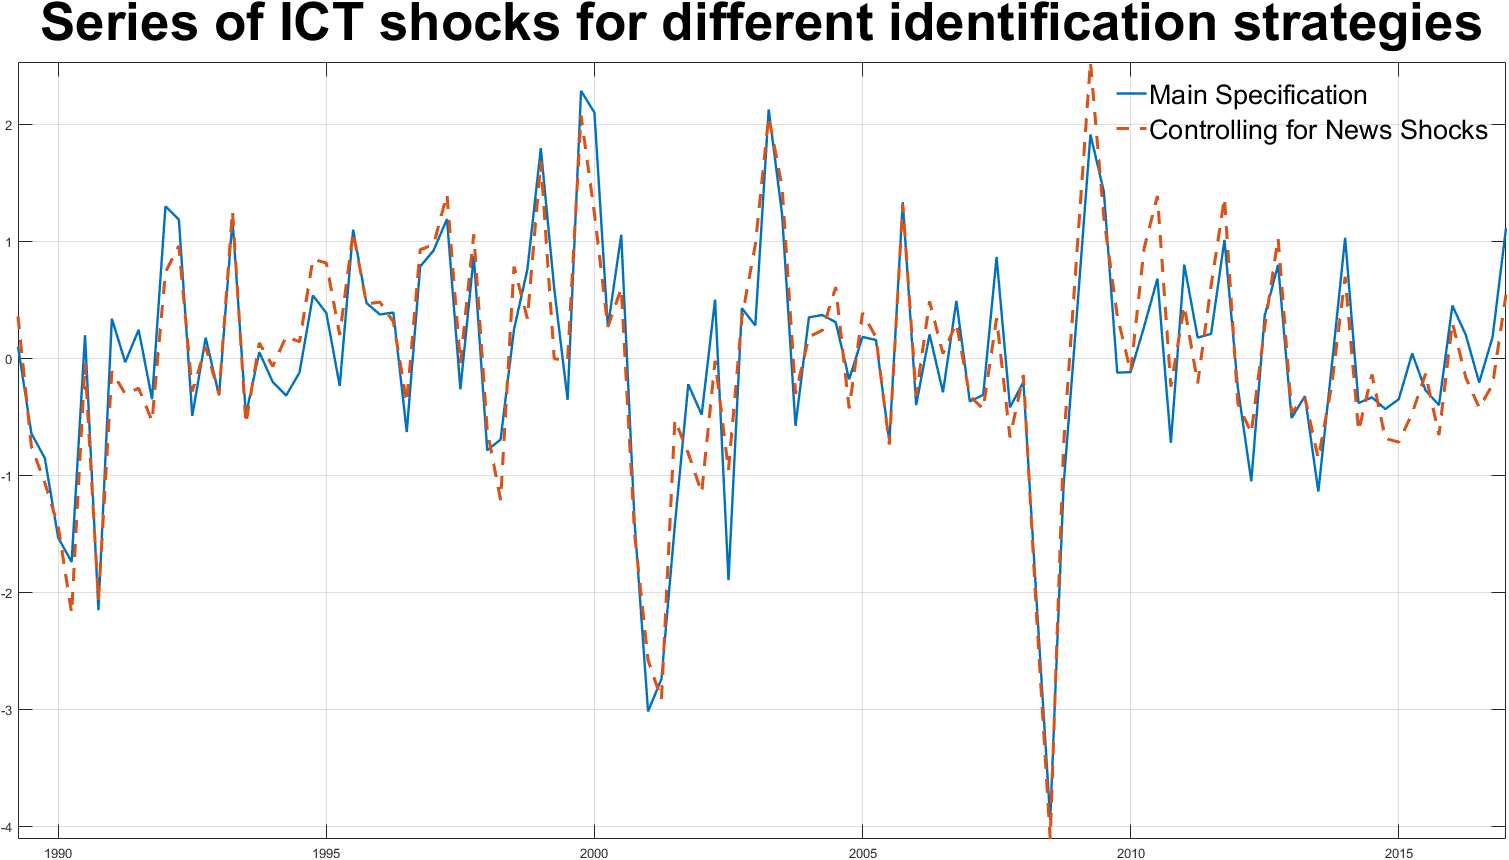
\includegraphics[scale=0.35]{MainFigures/ICTshocksSeries_ControllingforNEWS}
		\caption{ICT shock series using two different empirical strategy. Blue solid line represents shock series for the 5-dimension system \ref{eq:mainSpecification} presented in \ref{section:mainSpec}. Red dotted line represents shock series for the 6-dimensional system \ref{eq:newsSpecification} presented in \ref{section:twosteps} where we employ a 2-step identification strategy in order to control for news shocks.}
		\label{fig:shockSeries_2steps}
	\end{center} 
\end{figure}

\newpage

\section{Estimated Parameters via IR Matching}\label{sec:appendix_table_IRmatching}

 	\begin{table}[h!]
	\begin{center}
		\begin{tabular}{clc}
			\hline
			Symbol & Economic Interpretation & Estimated Value \\
			\hline
            $\sigma^2_{\iota}$ & Variance of ICT technological shock &   $0.01^2$  \\
            $\rho_{\iota}$     & Persistence of ICT technological shock & $0.9$   \\
            $\gamma$           & Size of spillover of ICT capital on TFP &  $0.5881$ \\
			\hline
		\end{tabular}
		\caption{Estimation of key parameters by imposing model's impulse responses of an ICT shock to be as close as possible to the empirical ones. Theoretical estimates are impulse responses to an ICT-specific technological shock, $\zeta_t$ which are functions of key parameters: $\sigma_{\iota}^2$, $\rho_{\iota}$, and $\gamma$. Empirical impulse responses of an ICT shock to TFP, ICTI, consumption, and relative prices are derived from Specification \ref{eq:mainSpecification} using the empirical strategy presented in Section \ref{section:empiricalstrategy_simple}. According to what presented in Appendix \ref{section:mainSetResults}, we use a horizon of $40$ periods for each response.}
		\label{table:estimated_parameters}
	\end{center}
\end{table}


\newpage

\section{Impulse-Response Matching}\label{section:appendix_IR_matching}
 
\begin{figure}[h!]
	\begin{subfigure}{.5\textwidth}
		\centering
		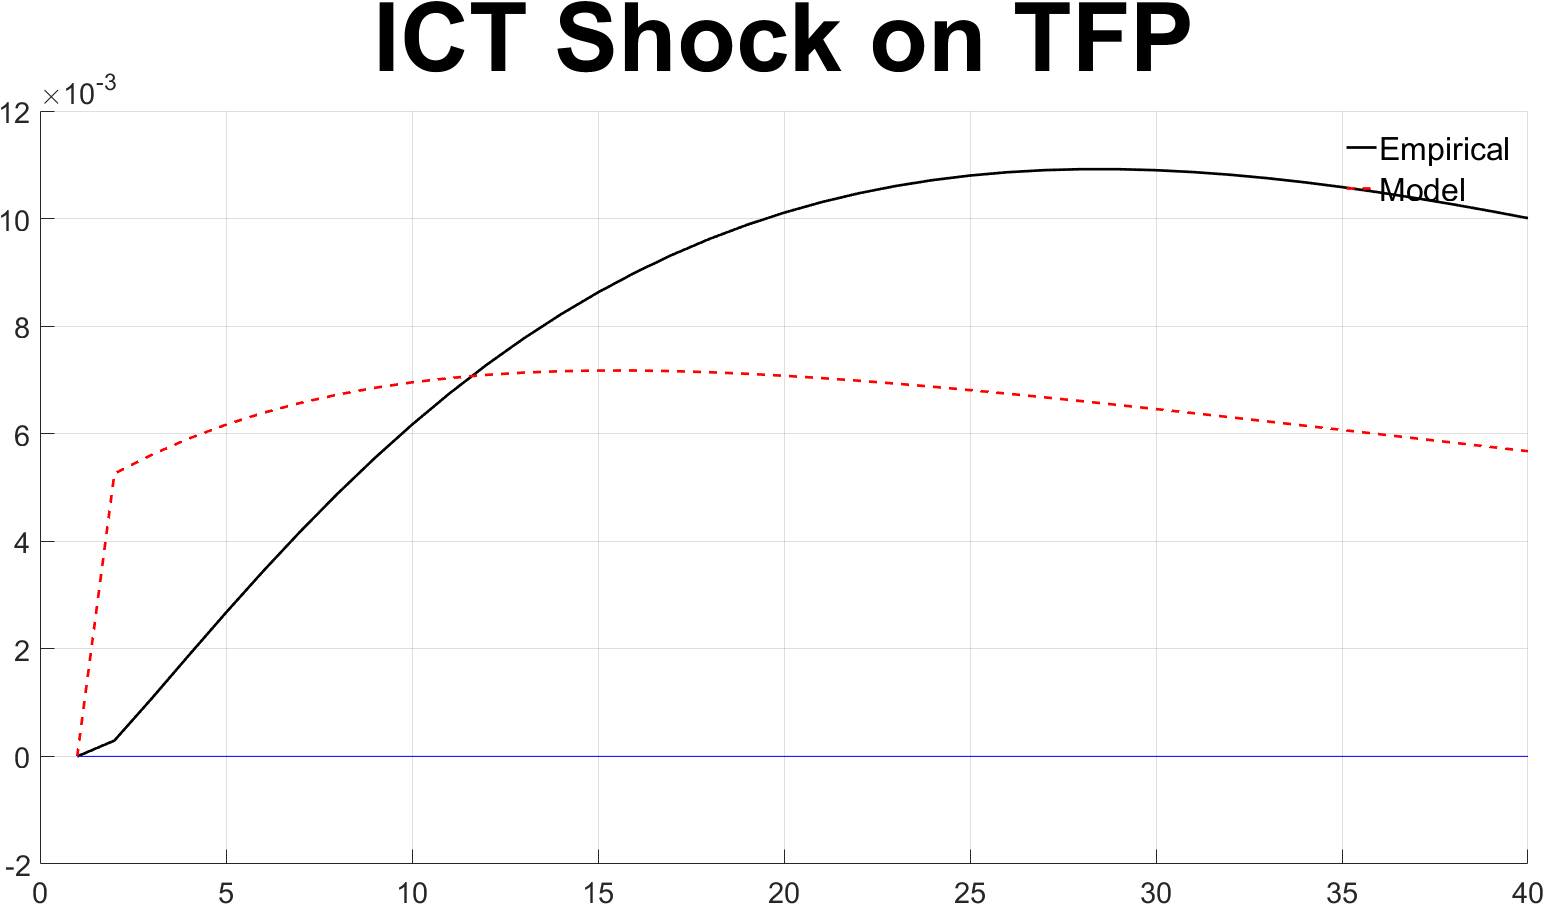
\includegraphics[width=1\linewidth]{MainFigures/fig_ICT_Shock_on_TFP_IRmatching_together}
	\end{subfigure}%
	\begin{subfigure}{.5\textwidth}
		\centering
		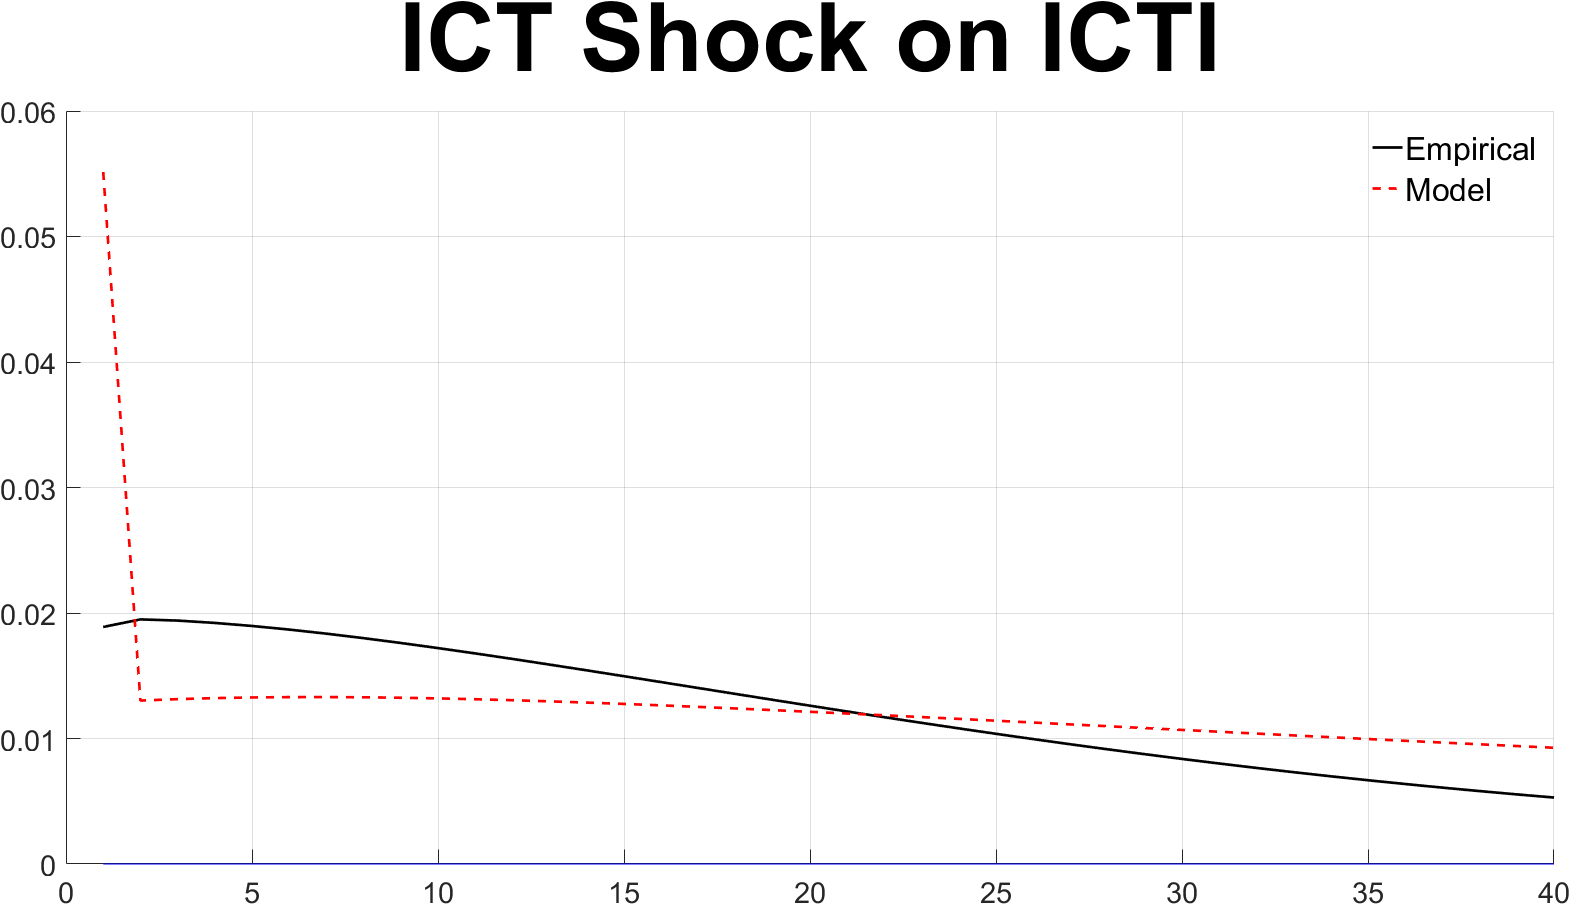
\includegraphics[width=1\linewidth]{MainFigures/fig_ICT_Shock_on_ICTI_IRmatching_together}
	\end{subfigure}
	%%%%%%%%%%%%%%%%%%%%%%%%%%%%%%%%%%%%%%%%%%%%%%%%%%%%%%%%%%%%
	\begin{subfigure}{.5\textwidth}
		\centering
		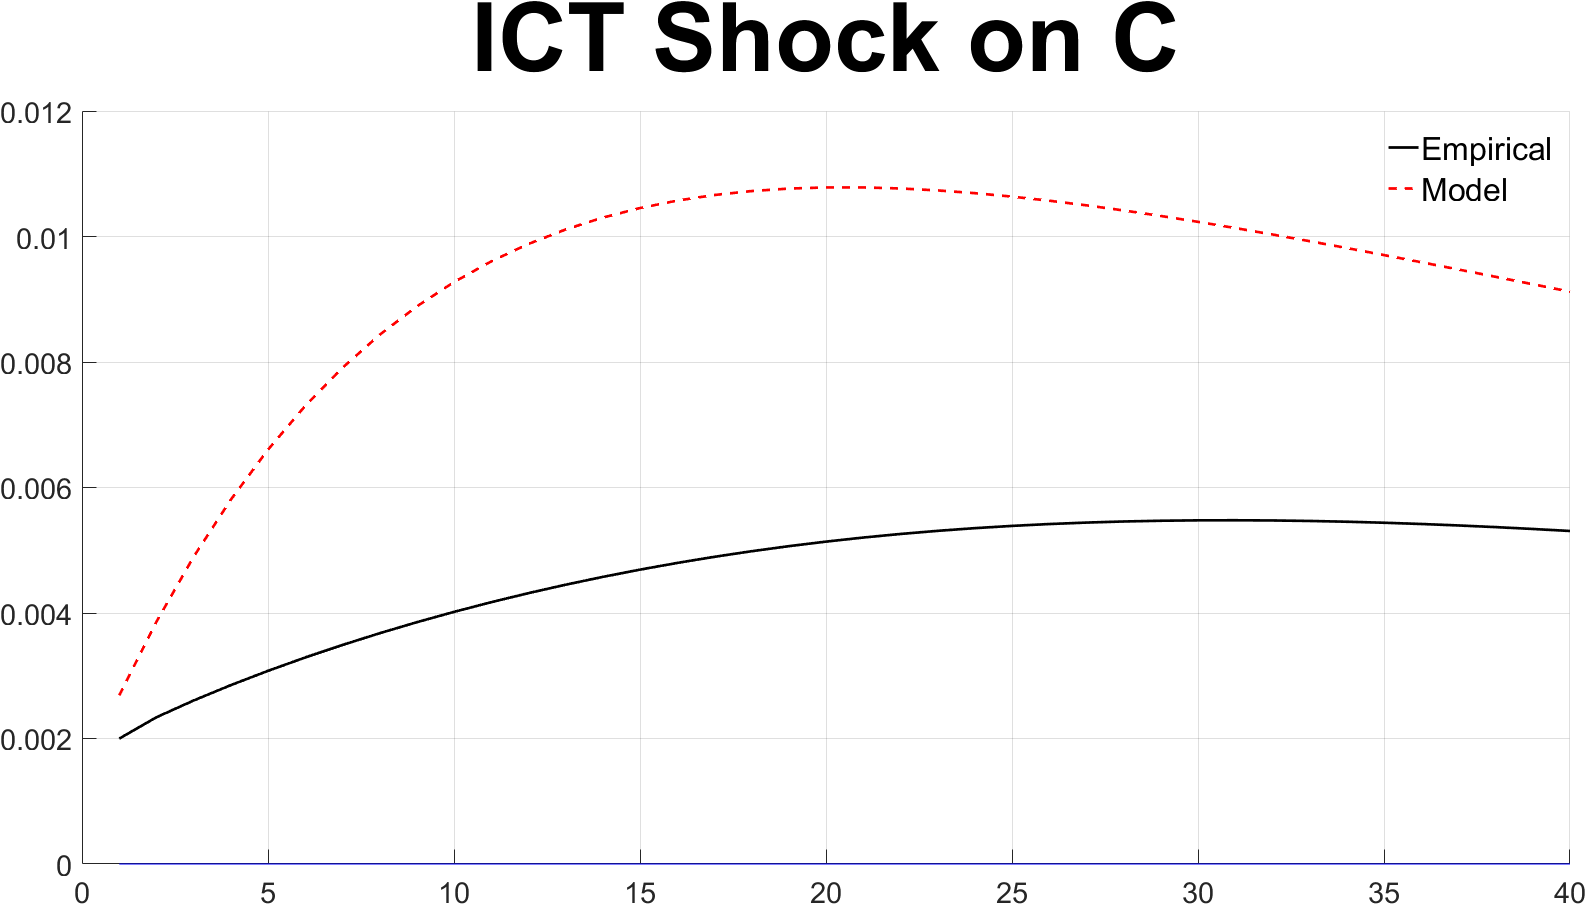
\includegraphics[width=1\linewidth]{MainFigures/fig_ICT_Shock_on_C_IRmatching_together}
	\end{subfigure}%
	\begin{subfigure}{.5\textwidth}
		\centering
		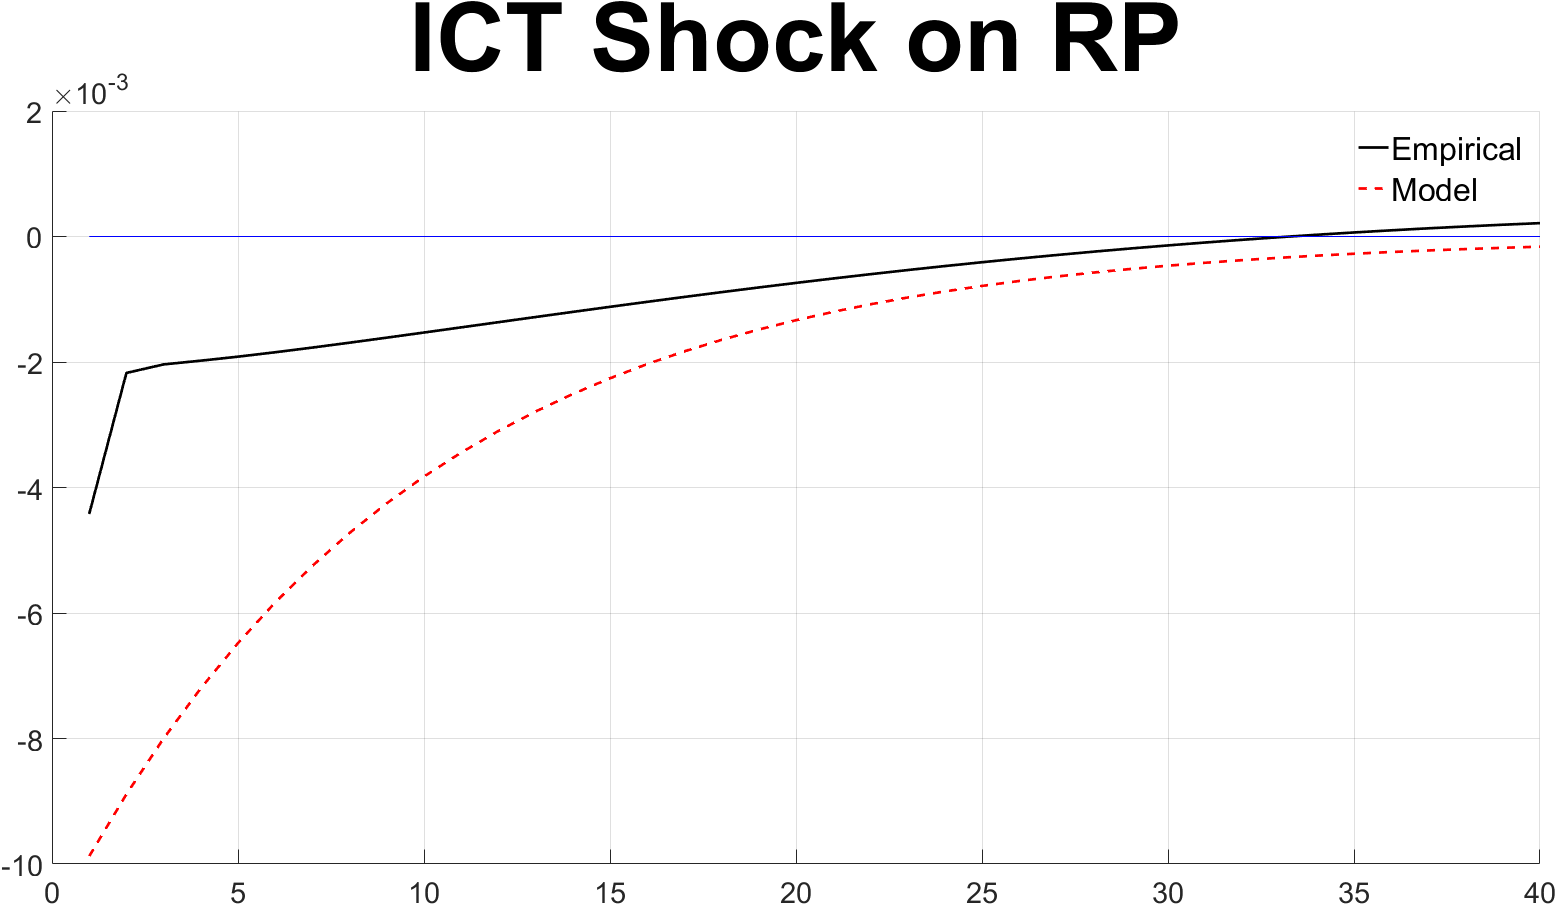
\includegraphics[width=1\linewidth]{MainFigures/fig_ICT_Shock_on_RP_IRmatching_together}
	\end{subfigure}
	%%%%%%%%%%%%%%%%%%%%%%%%%%%%%%%%%%%%%%%%%%%%%%%%%%%%%%%%%%%%
	\caption{Empirical VAR versus model responses to an ICT shock. The black solid lines show the empirical responses to an identified ICT shock in Specification \ref{eq:mainSpecification}. The dotted red lines show the model’s responses to a shock to the ICT-specific technological component $\zeta_t$. The horizontal axes refer to forecast horizon and the units of the vertical axes are percentage deviations.}
	\label{fig:IR_matching}
\end{figure}

 
\end{document}


